\chapter{\uppercase {Construction-D Lattices via Spatially coupled LDPC codes}\footnote{\textcopyright ~2014 IEEE. Reprinted, with permission, from A. Vem, Y.-C. Huang, K. R. Narayanan, H. D. Pfister, ``Multilevel lattices based on spatially-coupled LDPC codes with applications", International Symposium on Information Theory, 2014.}}
\label{chap:SCLDPClattices}

\def \figures_path{./data/SCLDPC}
Lattices have been studied in pure mathematics for more than two centuries. In the last few decades lattices have also found application in connection with coding theory, cryptography and various physical sciences. Codes derived from well designed lattice structures have been shown to be optimal coding solutions to several problems in information and coding theory \cite{erez05,zamir2014lattice}. In most of these cases, the underlying lattices are constructed using Construction-A and it has been shown that such lattices are simultaneously good for shaping (Roger's good) and for channel coding (Poltyrev good) \cite{erez05}. There are two important drawbacks in using optimal lattices constructed using Construction-A. On the theoretical side, the use of non-binary codes makes it difficult to prove the optimality of these lattices and lattice codes under practical decoding algorithms such as belief propagation (BP) decoding and so far, we are not aware of any results showing the optimality of Construction-A lattices under BP decoding. On the practical side, optimal lattices constructed from Construction-A typically require the underlying linear codes to work over large fields and hence, result in formidable decoding complexity, even with BP decoding.

In this chapter \cite{vem2014multilevel}, we discuss Construction-D lattices. We propose a class of lattices constructed using Construction-D \cite{BarnesSloane83} where the underlying linear codes are nested binary spatially-coupled low density parity check codes (SC-LDPC) codes with uniform left and right degrees. Forney {\em et al} \cite{forney2000} showed that the Construction-D lattices achieve the Poltyrev-limit under multi-stage decoding if the underlying codes at each level are capacity achieving. Leveraging this result, and the result due to Kudekar \textit{et al} proving that the regular SC-LDPC codes can universally achieve capacity under BP decoding for the class of binary memoryless symmetric (BMS) channels \cite{kudekaruniversal,kumar2014threshold}, we show that the proposed Construction-D lattices achieve the Poltyrev limit under multistage BP decoding.

 We refer to the proposed lattices as SC-LDPC lattices. The density evolution thresholds show that the proposed SC-LDPC lattices can approach the Poltyrev limit to within 0.2 dB under multistage BP decoding. Around the same time, binary polar codes have been used in conjunction with Construction-D to obtain Poltyrev-good lattices in \cite{YanLingWu13}. The focus of this chapter is on the use of SC-LDPC codes.

We then derive lattice codes from the proposed SC-LDPC lattices and apply them to the symmetric interference channel \cite{jafar10}.  It has been pointed out in \cite{Estela13} that there is a natural connection between lattices generated by Construction-D (or Construction-D$^\prime$) and the interference alignment scheme in \cite{jafar10}. In fact we observe that the interference alignment can be achieved by replacing the Barnes-Wall lattices in \cite{Estela13} by our proposed SC-LDPC lattices. Our numerical simulation results show that the proposed solution leads to a significant gain in terms of error probability performance. 
%This class of lattice codes can also be applied to Integer-forcing or compute-and-forward in the multiple access stage \cite{nazer2011CF}.

Throughout the rest of the chapter, vectors and matrices are written in lowercase boldface and uppercase boldface, respectively. $\mbf{I}_{n}$ denotes identity matrix of size $n\times n$.

\section{Lattices: Review}\label{Section:Background}
A lattice $\Lmb$ is a discrete set of points in Euclidean space that form an additive group. More precisely an $m$-dimensional lattice $\Lmb^{(n)}\subset \R^{n}$ can be defined as:
\begin{equation}
\Lmb^{(n)} =\{\lmb\in\R^{n}:\lmb=\mathbf{M}\mbf{u},\mbf{u}\in \Z^{m}\}
\end{equation}
where $\mathbf{M}\in\R^{n \times m}$ is full-rank and is called the generator matrix of the lattice. Throughout this chapter, whenever a lattice $\Lmb$ is used without the superscript, it is understood that the lattice is contained in the $n$-dimensional Euclidean space i.e., $\Lmb\subset \R^{n}$. For a given lattice $\Lmb$, we denote the \tit{quantizer} with respect to the lattice as $Q_{\Lmb}$,  \tit{modulo} operation with respect to the lattice as $\mod \Lmb$,  \tit{fundamental Voronoi region} as $\mc{V}_{\Lmb}$ and the \tit{fundamental volume} defined as the volume of any fundamental region as Vol$(\Lmb)$. For more details on the lattice terminology see \cite{zamir2014lattice}.

Assume that some $\mbf{\lmb}\in\Lmb$ is transmitted through an additive white Gaussian noise (AWGN) channel of variance $\sigma^{2}$. The \textit{volume-to-noise ratio}(VNR) of $\Lmb$, $\alpha^{2}(\Lmb,\sigma^{2})$, is defined as:
\begin{equation}\label{Eqn:VNRDefinition}
\alpha^{2}(\Lmb,\sigma^{2})=\frac{\text{Vol}(\Lmb)^{2/n}}{2\pi e\sigma^{2}}.
\end{equation}

At the receiver given the decoder $\mc{D}:\mbb{R}^{n}\rightarrow\Lmb$, let us denote the error probability of decoding a lattice point $\lmb\in\Lmb$ as $\tx{P}(\mathbf{\lmb},\sigma^{2})$ under decoder $\mc{D}$. To be more precise,  %we define $\tx{P}(\mathbf{\lmb},\sigma^{2})$ as
\begin{equation*}
 \tx{P}(\mathbf{\lmb},\sigma^{2}):=\Pr\left(\mc{D}(\mathbf{\lmb}+\mathbf{z})\neq  \lmb\right),
\end{equation*}
where the noise vector is denoted by $\mbf{z}$.
%where $d(\mathbf{x},\mathbf{y})$ is the Euclidean distance between $\mathbf{x}$ and $\mathbf{y}$. 
For an infinite lattice $\Lmb$, $\tx{P}(\lmb,\sigma^{2})$ under the minimum Euclidean distance decoder is independent of $\lmb$ and hence the average probability of decoding error for the lattice  $\tx{P}(\Lmb,\sigma^{2})$ is the same as $\tx{P}(\lmb,\sigma^{2})$ for any $\lmb\in \Lmb$. Note that minimum distance decoder is the optimal decoder for this problem.
% \tx{P}(\mathbf{\lmb},\sigma^{2}):=\Pr\left(d(\mathbf{\lmb},\mathbf{\lmb}+\mathbf{z})\geq d(\mathbf{\lmb'},\mathbf{\lmb'}+\mathbf{z}) \text{ for any } \mathbf{\lmb'}\in\Lmb\right),

\subsection{Poltyrev limit}
\begin{definition}[Poltyrev Limit]\label{Def:PoltyrevLimit}
Poltyrev in \cite{poltyrev94} showed that for any $\delta>0$ there exists sequence of lattices $\Lmb^{(n)}$, indexed by $n$, such that the volume-to-noise ratio $\alpha^{2}(\Lmb^{(n)},\sigma^{2})<1+\delta,~ \forall n$ and the average error probability under minimum distance decoder $\tx{P}(\Lmb^{(n)},\sigma^{2}) \rightarrow 0$ as $n \rightarrow \infty$. We shall call such a sequence of lattices as being Poltyrev-good.
\end{definition}
\begin{remark}
The converse to the Poltyrev limit i.e., if the VNR of any lattice $\Lmb$, $\alpha^{2}(\Lmb,\sigma^{2})<1$, then it can be shown by simple geometric arguments that the average probability of decoding error is bounded away from $0$ even under the minimum distance decoder. Thus the Poltyrev limit is a fundamental limit for the unconstrained AWGN channel coding problem. And also note that to show that a specific sequence of lattices achieve Poltyrev limit it suffices to show that the sequence of lattices satisfy the conditions in Definition \ref{Def:PoltyrevLimit} using any decoder, not necessarily the optimal minimum distance decoder.
\end{remark}

\subsection{Construction-D and its goodness}
In the literature, even though many lattice constructions such as Construction-A, Construction-D, Construction-D$^\prime$, Construction E etc.., were available  since the 1960s, we can safely say that Construction-A has been the most popular one among the information and coding theory communities. The main reason being that the lattices based on Construction-A are used to show (constructive) optimal solutions to various problems like sphere packing, covering, channel coding, source coding, physical-layer network coding etc., \cite{nazer2011CF,erez05,sridharan2008capacity,Estela13}. Note that in many of these applications, the optimality is only asymptotic in the field size over which the Construction-A lattice is constructed upon. So even though the Construction-A provides us optimal lattices, the main disadvantage is that at the encoder and decoder should operate over finite fields of very large size. However Construction-D with it's multi-level structure enables us to work over fields of very small size at each level thus making Construction-D lattices much more amenable for practical implementation.

 In this subsection we briefly describe multilevel construction of lattices \cite{BarnesSloane83,conwaysphere}, specifically Construction-D and then recall Forney {\em et al}'s result on the existence of Poltyrev-good lattices based on this construction \cite{forney2000}.

Multilevel construction of lattices is based on a sequence of nested codes $\{\mathcal{C}_{l},1\leq l\leq r\}$ where each code $\mathcal{C}_{l}$ is of length $n$ over $\mathbb{F}_q$, a field of size $q$. Construction-D and Construction-D$^{\prime}$ are based on such nested sequence of linear codes. For details we refer the reader to \cite{conwaysphere}. Throughout this work we work with binary linear codes i.e., $q=2$. For $1\leq i \leq r$ where $r$ is the number of levels, let $\mathcal{C}_{i}$ be a $(n,k_i)$ binary code spanned by the set of binary $n$-tuples $\{\mathbf{g}_1,\mathbf{g}_2,\ldots,\mathbf{g}_{k_i}\}$ linearly independent over $\Z$ where $k_{1}\leq k_{2}\leq \cdots \leq k_{r}$. One can observe that $\mc{C}_{1}\subseteq \ldots \subseteq \mc{C}_{2}\subseteq \mc{C}_{r}$. Using such nested binary linear codes $\{\mathcal{C}_{j},1\leq j\leq r\}$, a multilevel Construction-D lattice $\Lmb$ can be defined as follows:
\begin{align}\label{Eqn:ConstrD}
 \Lmb=\biggl\{2^{r}\Z^{n}+\sum_{1\leq i\leq r}2^{i-1}\sum_{1\leq j\leq k_{i}}\alpha_{ij}\mathbf{g}_j|\alpha_{ij}\in\{0,1\}\biggr\}
\end{align}
where ``$+$" denotes addition in $\R^{n}$.  Since the generator vectors $\mbf{g}_{1},\mbf{g}_{2},\ldots,\mbf{g}_{k_{r}}$ are all linearly independent and based on the fact that the volume of the Voronoi region corresponding to each point in the lattice is equal to the 	volume of the fundamental Voronoi region, the VNR of a Construction-D lattice described in \eqref{Eqn:ConstrD} can be computed to be
\begin{equation}\label{Eqn:VNRConstrutionD}
    \alpha^{2}(\Lmb,\sigma^{2})=\frac{2^{2(r-\sum_{i=1}^{r}k_{i}/n)}}{2\pi e\sigma^{2}}.
\end{equation}

\subsubsection*{Multistage Decoder}
We describe the multistage decoding that can be used to decode a Construction-D lattice over any memoryless additive noise channel. Let $\lmb\in\Lmb$, where $\Lmb$ is as defined in \eqref{Eqn:ConstrD}, be transmitted through an AWGN channel and $\mathbf{y}=\lmb+\mathbf{z}$ is received where $\mathbf{z}\sim\mathcal{N}(0,\sigma^{2} \mbf{I}_{n})$. Let $\mc{D}_{i}$ be the component decoder corresponding to $\mc{C}_{i}$ which, given any $\mbf{x}\in\R^{n}$, maps it to a codeword in $\mc{C}_{i}$, i.e., $\mc{D}_{i}(\mbf{x})\in\mc{C}_{i}$. Let the initialization step be $\hat{\mathbf{y}}_{0}=\mathbf{y}$.
\begin{itemize}
\item \tit{Step} 1: At stage $i, $ $1\leq i\leq r$, $\hat{\mathbf{y}}_{i-1}\mod 2$ is decoded to a codeword  $\hat{\mathbf{x}}_{i}\in \mathcal{C}_{i}$. Also, the corresponding information bits  $\{\hat{\alpha}_{i1},\hat{\alpha}_{i2},\ldots, \hat{\alpha}_{ik_{i}}\}\in \{0,1\}^{k_{i}}$ that generate $\hat{\mathbf{x}}_{i}$, are computed.
\item \tit{Step} 2: Compute $\hat{\mathbf{y}}_{i}= \frac{1}{2} \cdot(\hat{\mathbf{y}}_{i-1}-\sum_{1\leq i\leq k_{i}}\hat{\alpha}_{ij}\mathbf{g}_j)$. Go to \tit{Step} 1.
%\vspace{2pt}
\item \tit{Step} 3: At $(r+1)^{\text{th}}$ stage of decoding, $\hat{\mathbf{y}}_{r}$ is decoded to the closest $\mathbf{q}\in\Z^{n}$ with respect to the Euclidean norm.
%\vspace{2pt}
\item \tit{Output}: Decoded lattice point $\hat{\mathbf{\lmb}}\in\Lmb$ is given by
\begin{align}
    \hat{\mathbf{\lmb}}=2^{r}\mathbf{q}+\sum_{1\leq i\leq r}2^{i-1}\sum_{1\leq j\leq k_{i}}\hat{\alpha}_{ij}\mathbf{g}_{j}.
\end{align}

\end{itemize}

At the $i^{\text{th}}$ stage of decoding, conditioned on successful decoding in previous stages i.e., assuming $\hat{\alpha}_{pj}=\alpha_{pj}$ for $1\leq p < i$, the input to the decoder is of the form
\begin{align}
\hat{\mathbf{y}}_{i-1}\! \mod 2&\equiv\frac{1}{2}\Big(\hat{\mathbf{y}}_{i-2}-\sum_{1\leq j\leq k_{i-1}}\alpha_{(i-1)j}\mathbf{g}_j\Big)\!\mod 2\notag\\
&\equiv \Big( \frac{1}{2^{i-1}}\hat{\mathbf{y}}_{0}-\sum_{1\leq p< i}2^{p-i}\sum_{1\leq j\leq k_{p}}\alpha_{pj}\mathbf{g}_j \Big) \hspace{-8pt}\mod 2\notag\\
&\equiv\frac{1}{2^{i-1}}\Big( \mathbf{y}-\sum_{1\leq p< i}2^{p-1}\sum_{1\leq j\leq k_{p}}\alpha_{pj}\mathbf{g}_j \Big) \hspace{-8pt}\mod 2\notag\\
&\equiv\Big(\sum_{j=1}^{k_{i}}\alpha_{ij}\mathbf{g}_j \Big) \hspace{-8pt}\mod 2 + \Big( 2^{-(i-1)}\mathbf{z} \Big) \hspace{-8pt}\mod 2\notag\\
&\equiv\mathbf{x}_{i}+2^{-(i-1)}\mathbf{z} \hspace{-8pt}\mod 2,
\label{Eqn:Mod2Channel}
\end{align}
where $\mathbf{x}_{i}\in\mathcal{C}_{j}$. We call the channel defined in \eqref{Eqn:Mod2Channel} as an additive mod-2 Gaussian noise (AMGN) channel \cite{forney2000} and denote the capacity for this channel as  $\text{C}_{\text{AMGN}}(\sigma^{2}_{i})$ where $\sigma_{i}^{2}=2^{-2(i-1)}\sigma^2$.

\begin{theorem}[Forney \textit{et al.} \cite{forney2000}]
For an AWGN channel with noise variance per dimension $\sigma^{2}$, there exists a sequence of Construction-D lattices $\Lmb$ based on a chain of $r$ two-way one-dimensional lattice partitions and $r$ nested random binary linear codes $\mathcal{C}_{1}\subseteq \mathcal{C}_{2}\cdots \subseteq \mathcal{C}_{r}$ that is Poltyrev-good.
\end{theorem}

\begin{remark}\label{Rmk:Forney_proof}
    Note that in \cite{forney2000}, it was shown that if for each level $j\in\{1,\ldots,r\}$ the binary linear code $\mathcal{C}_{j}$ at that respective level is arbitrarily close to the capacity of the respective AMGN channel and has an arbitrarily low error probability in that stage of the multistage decoder then it was shown that the Construction-D lattice can thus be constructed arbitrarily close to the Poltyrev-limit with an arbitrarily low probability of error.
\end{remark}

\section{Proposed SC-LDPC Lattices}\label{Sec:SCLDPC}
As we can see from $\eqref{Eqn:ConstrD}$, construction of lattices based on Construction-D using SC-LDPC codes requires the spanning sets, or equivalently generator matrices, of the respective codes to be nested. In other words we need a sequence of SC-LDPC codes where each code is nested in the next code of the sequence. In this section, we first construct such a sequence of nested linear codes where each code has the structure similar to a SC-LDPC system and hence has good error performance at rates arbitrarily close to Shannon capacity. For ease of exposition, we restrict our description to the case $r=2$. For higher values the construction extends naturally.

\subsection{Construction}
Let the required rates of the two codes be $r_{1}$ and $r_{2}$, $0< r_{1}<r_{2}$. Prior to the details, let us recall that the Tanner graph of a rate $\frac{k}{n}$ binary linear code is the bipartite graph whose $n-k$ check nodes represent the parity check equations defining the code and the $n$ variable nodes represent the bits of the code. Our objective is to construct Tanner graphs $\mc{G}_{1},\mc{G}_{2}$ similar in structure to a SC-LDPC system(reference needed?) such that the binary codes $\mc{C}_{1},\mc{C}_{2}$ represented by the respective graphs are nested i.e., $\mc{C}_{1}\subseteq \mc{C}_{2}$ and the rates are arbitrarily close to $r_{1}$ and $r_{2}$ respectively. For small enough $\epsilon >0$, choose $d_{c}\in\N$ such that there exists $d_{v}^{1},d_{v}^{2}\in \N$,
\begin{align}
	d_{v}^{i}\geq 3 \hspace{0.3cm} \text{  and }  \hspace{0.3cm}  1-\frac{d_{v}^{i}}{d_{c}}>r_{i}-\epsilon, i\in \{1,2\}.
						\label{Eqn:DegreeConditions1}
\end{align}
The $\epsilon$ leeway in the above equations is just for rounding off $r_{i}$ to the nearest rational number and not very significant.
\iflonger
 [ALSO WHY THE BIT NODE DEGREE SHOULD BE ATLEAST 3].
 \fi

In this approach we first construct a regular $(d_{v}^{1},d_{c})$ Tanner graph $\mc{G}_{1}$ where regularity here means that all the variables have degree $d_{v}^{1}$ and all checks have degree $d_{c}$. Then we obtain the Tanner graph $\mc{G}_{2}$ by removing a fraction of the parity checks and the edges incident on these checks in a systematic fashion that $\mc{G}_{2}$ is $(d_{v}^{2},d_{c})$ regular. The ensemble described in \cite{KudekarUrbanke11} is not directly amenable to our approach of deriving the higher rate code, since removing a fraction of the checks from this ensemble does not result in a regular SC-LDPC code. Therefore, our approach is to use the following multi edge-type construction.

Fix $M\in \N$. We place $M d_{c}$ variable nodes at each position in the range $[1: L]\coleq\{1,2,\ldots ,L\}$, $L\in\N$ and $Md_{v}^{1}$ check nodes at each position in the range $[1 : L+w-1]$, where $w\in \N$ is coupling width. At each position divide the $Md_{v}^{1}$ check nodes into $d_{v}^{1}$ groups where each group contains $M$ check nodes. At any position we refer to all check nodes belonging to $k^{\text{th}}$ group as of type $\mc{T}_{k}$. This equates to, at each position,  $Md_{c}$ edges coming from check nodes of type $\mc{T}_{k}$ for all $k\in [1:d_{v}^{1}]$. Similarly, for each variable node, we arbitrarily classify the $d_{v}^{1}$ edges into types, where $k^{\text{th}}$ edge is referred to as type $\mc{E}_{k}$ which equates to $Md_{c}$ edges of each type at any position. For a fixed $k \in [1 : d_{v}^{1}]$, for all $i \in [1 : L]$, each edge of type $\mc{E}_{k}$ at position $i$ is assigned uniformly at random to a type $\mc{T}_{k}$ check node from positions $[i : i+w-1]$. The main idea is that, for each $k\in [1:d_{v}^{1}]$, if we consider the sub-graph containing only the type $\mc{T}_{k}$ check nodes and variable nodes with single edge (type $\mc{E}_{k}$ edges) the above mimics the construction of a $(1,d_{c},L,w)$ ensemble \cite{KudekarUrbanke11} on the sub-graph. This results in a Tanner graph in which every variable node has exactly one edge connected to type $\mc{T}_{k}$ check node, for all $k \in [1: d_{v}^{1}]$. We call such a graph, a \textit{check-uniform connected graph}.

More precisely, the ensemble is defined as follows. Choose $M$ such that $\frac{Md_{c}}{w}$ is a natural number. Fix $k\in[1:d_{v}^{1}]$ and $i\in[1:L]$. Choose a permutation $\pi^{v}_{i,k}$ uniformly at random from the set of permutations on $Md_{c}$ letters. Under arbitrary indexing of the $Md_{c}$ variable nodes at position $i$, for $j\in [0:w-1]$, assign $\mc{E}_{k}$ type edges of $\pi^{v}_{i,k}\left(j\frac{Md_{c}}{w}+1:(j+1)\frac{Md_{c}}{w}\right)$ variable nodes at position $i$ to check nodes at position $i+j$. Under this assignment, ignoring the boundary effects, for each check node type at position $i+j$, the number of edges that come from variable nodes at position $i$ is $\frac{Md_{c}}{w}$, a $w^{\text{th}}$ fraction of the total number of connections. From the check nodes perspective, for $k\in[1:d_{v}^{1}]$, at  each position, distribute these edges according to a permutation $\pi^{c}_{i,k}$ chosen uniformly at random from the set of all permutations on $Md_{c}$ letters. We call the proposed construction as $(d_{v}^{1},d_{c},L,w)$ \textit{check-uniform} SC-LDPC (CU-SC-LDPC) ensemble of codes.  

Choose a Tanner graph uniformly at random from the above described $(d_{v}^{1},d_{c},L,w)$ CU-SC-LDPC ensemble, call it $\mc{G}_{1}$. Observe that, removal of all check nodes of a particular type, say $\mc{T}_{d_{v}^{1}}$, from $\mc{G}_{1}$ results in a regular $(d_{v}^{1}-1,d_{c})$ Tanner graph. One can see that removal of all check nodes of types $\mc{T}_{d_{v}^{2}+1},\mc{T}_{d_{v}^{2}+2},\ldots, \mc{T}_{d_{v}^1} $ from $\mc{G}_{1}$ results in a graph from the $(d_{c},d_{v}^{2},L,w)$ CU-SC-LDPC ensemble, which let's refer to as $\mc{G}_{2}$. More importantly, all the check-nodes in the derived graph $\mc{G}_{2}$ are also contained in $\mc{G}_{1}$ and hence any codeword satisfying all the check constraints in $\mc{G}_{1}$ also satisfies all the check constraints in $\mc{G}_{2}$. Thus we can say that the binary code $\mc{C}_{1}$ defined by $\mc{G}_{1}$ is a sub-code of the binary code $\mc{C}_{2}$ defined by $\mc{G}_{2}$. One can obtain a sequence of nested linear codes $\mc{C}_1\subseteq\mc{C}_2\subseteq\ldots\mc{C}_r$ by repeatedly performing the above operation. Given $(d_{c},d_{v}^{1},\ldots,d_{v}^{r})$, for each code $\mc{C}_{1}$ from the $(d_{c},d_{v}^{1},L,w)$ CU-SC-LDPC ensemble, we can obtain a nested sequence of codes $\mc{C}_1,\mc{C}_2,\ldots,\subseteq\mc{C}_r$ where $\mc{C}_{i} \in (d_{c},d_{v}^{i},L,w)$ CU-SC-LDPC ensemble.  We call the proposed ensemble of nested sequences of codes as $(d_{c},d_{v}^{1},\ldots,d_{v}^{r},L,w)$ CU-SC-LDPC ensemble. 

\begin{figure}[ht!]
\centering
\resizebox {0.9\textwidth}{!} {
\begin{tikzpicture}[]

\draw [pattern=north west lines, pattern color=blue] (0.1,0.1) rectangle (-0.1,-0.1); \node [left,font=\tiny] at (0.03,0){$\mc{T}_{1}$} ;
\draw [fill=black] (0.1,0.1) rectangle (-0.1,-0.1); 
\node [left,font=\tiny] at (0.03,0){$\mathcal{T}_{1}$} ;

	\draw[thick,black] (0,2) circle (0.1);  \draw[thick,black] (0,-2) circle (0.1);
	\draw[thick,black] (0.6,0.1) rectangle (0.4,-0.1);\node [left,font=\tiny] at (0.52,0){$\mathcal{T}_{2}$} ;
  	\draw[thick,black] (0.5,2) circle (0.1);  \draw[thick,black] (0.5,-2) circle (0.1);
	\draw[thick,black] (1.1,0.1) rectangle (0.9,-0.1); \node [right,font=\tiny] at (0.97,0){$\mathcal{T}_{3}$} ;
 	\draw[thick,black] (1,2) circle (0.1);  \draw[thick,black] (1,-2) circle (0.1);

\draw [dashed] (0,1.9) -- (0,0.1);  \draw (0,1.9) -- (2.5,0.1); \draw (0,1.9) -- (1,0.1);
\draw [dashed] (0.5,1.9) -- (0,0.1);  \draw (0.5,1.9) -- (0.5,0.1); \draw (0.5,1.9) -- (3,0.1);
\draw [dashed] (1,1.9) -- (2,0.1);  \draw (1,1.9) -- (0.5,0.1); \draw (1,1.9) -- (3,0.1);

\draw [dashed] (0,-1.9) -- (2,-0.1);  \draw (0,-1.9) -- (2.5,-0.1); \draw (0,-1.9) -- (1,-0.1);
\draw  [dashed] (0.5,-1.9) -- (0,-0.1);  \draw (0.5,-1.9) -- (2.5,-0.1); \draw (0.5,-1.9) -- (1,-0.1);
\draw [dashed] (1,-1.9) -- (2,-0.1);  \draw (1,-1.9) -- (0.5,-0.1); \draw (1,-1.9) -- (1,-0.1);

\draw [fill=black] (2.1,0.1) rectangle (1.9,-0.1);
\node [left,font=\tiny] at (2.03,0){$\mathcal{T}_{1}$} ;
\draw[thick,black] (2,2) circle (0.1);  \draw[thick,black] (2,-2) circle (0.1);
\draw[thick,black] (2.6,0.1) rectangle (2.4,-0.1); \node [left,font=\tiny] at (2.52,0){$\mathcal{T}_{2}$} ;
\draw[thick,black] (2.5,2) circle (0.1);  \draw[thick,black] (2.5,-2) circle (0.1);
\draw[thick,black] (3.1,0.1) rectangle (2.9,-0.1);  	\node [right,font=\tiny] at (2.97,0){$\mathcal{T}_{3}$} ;
\draw[thick,black] (3,2) circle (0.1);  \draw[thick,black] (3,-2) circle (0.1);
\draw [dashed] (2,1.9) -- (4,0.1);  \draw (2,1.9) -- (2.5,0.1); \draw (2,1.9) -- (3,0.1);
\draw [dashed] (2.5,1.9) -- (2,0.1);  \draw (2.5,1.9) -- (4.5,0.1); \draw (2.5,1.9) -- (3,0.1);
\draw [dashed] (3,1.9) -- (4,0.1);  \draw (3,1.9) -- (2.5,0.1); \draw (3,1.9) -- (5,0.1);

\draw [dashed] (2,-1.9) -- (2,-0.1);  \draw (2,-1.9) -- (2.5,-0.1); \draw (2,-1.9) -- (5,-0.1);
\draw (2.5,-1.9) -- (4,-0.1);  \draw (2.5,-1.9) -- (4.5,-0.1); \draw (2.5,-1.9) -- (3,-0.1);
\draw [dashed] (3,-1.9) -- (2,-0.1);  \draw (3,-1.9) -- (4.5,-0.1); \draw (3,-1.9) -- (3,-0.1);

\draw [fill=black] (4.1,0.1) rectangle (3.9,-0.1);  
\node [left,font=\tiny] at (4.03,0){$\mathcal{T}_{1}$} ;
   \draw[thick,black] (4,2) circle (0.1);  \draw[thick,black] (4,-2) circle (0.1);
\draw[thick,black] (4.6,0.1) rectangle (4.4,-0.1);  \node [left,font=\tiny] at (4.52,0){$\mathcal{T}_{2}$} ;
   \draw[thick,black] (4.5,2) circle (0.1);  \draw[thick,black] (4.5,-2) circle (0.1);
\draw[thick,black] (5.1,0.1) rectangle (4.9,-0.1);   \node [right,font=\tiny] at (5,0){$\mathcal{T}_{3}$} ;
 \draw[thick,black] (5,2) circle (0.1);  \draw[thick,black] (5,-2) circle (0.1);

\draw [dashed] (4,1.9) -- (6,0.1);  \draw (4,1.9) -- (4.5,0.1); \draw (4,1.9) -- (5,0.1);
\draw [dashed] (4.5,1.9) -- (4,0.1);  \draw (4.5,1.9) -- (4.5,0.1); \draw (4.5,1.9) -- (7,0.1);
\draw [dashed] (5,1.9) -- (6,0.1);  \draw (5,1.9) -- (6.5,0.1); \draw (5,1.9) -- (5,0.1);

\draw [dashed] (4,-1.9) -- (4,-0.1);  \draw (4,-1.9) -- (6.5,-0.1); \draw (4,-1.9) -- (5,-0.1);
\draw [dashed] (4.5,-1.9) -- (4,-0.1);  \draw (4.5,-1.9) -- (6.5,-0.1); \draw (4.5,-1.9) -- (5,-0.1);
\draw [dashed] (5,-1.9) -- (6,-0.1);  \draw (5,-1.9) -- (4.5,-0.1); \draw (5,-1.9) -- (7,-0.1);

\draw [fill=black] (6.1,0.1) rectangle (5.9,-0.1);
\node [left,font=\tiny] at (6.03,0){$\mathcal{T}_{1}$} ;
\draw[thick,black] (6.6,0.1) rectangle (6.4,-0.1); \node [left,font=\tiny] at (6.52,0){$\mathcal{T}_{2}$} ;
\draw[thick,black] (7.1,0.1) rectangle (6.9,-0.1);  \node [right,font=\tiny] at (6.97,0){$\mathcal{T}_{3}$} ;

 \end{tikzpicture} 

%\end{document}
}
\caption{A example Tanner graph from the $(3,6)$, $L=3$, $w=2$ CU-SC-LDPC ensemble. Removal of all the type $\mc{T}_{1}$ check nodes i.e the filled nodes, results in a $(2,6)$ CU-SC-LDPC protograph, see Fig.\ref{BaseGraph_sup}. }
\label{Basegraph}
\end{figure}


\begin{remark}\label{Rmk:EquivNestedConstr1}
Observe that choosing $\mc{G}_{1}$ uniformly at random from the $(d_{c},d_{v}^{1},L,w)$ CU-SC-LDPC ensemble is equivalent to choosing a set of permutations $\Pi_{1}=\{\pi_{i,k}^{c},\pi_{i,k}^{v}: i\in[1:L],k\in[1:d_{v}^{1}]\}$ where each permutation is chosen uniformly at random from the set of permutations on $Md_{c}$ letters. Deriving nested graph $\mc{G}_{2}$ is equivalent to considering just the subset: $\Pi_{2}=\{\pi_{i,k}^{c},\pi_{i,k}^{v}: i\in[1:L],k\in[1:d_{v}^{2}]\}$ of permutations. Hence this construction of nested codes is equivalent to first constructing $\mc{G}_{2}$ by choosing $\Pi_{2}$ and then choosing $\{\pi_{i,k}^{c},\pi_{i,k}^{v}: i\in[1:L], k\in[d_{v}^{2}+1:d_{v}^{1}]\}$ to construct $\Pi_{1}$ or equivalently $\mc{G}_{1}$.
\end{remark}

\begin{example}\label{Ex:ConstrD.1}
For $r_{1}=0.5$, $r_{2}=0.9$ let us try to compute the degree profiles satisfying \eqref{Eqn:DegreeConditions1}. One can see that      any triplet $(d_{c},d_{v}^{1},d_{v}^{2})=(10k, 5k, k), k\geq 3$, satisfies all the required conditions and $(30, 15, 3)$ is the simplest degree profile. We will see later the justification for choosing, $r_{2}=0.9$ in this example (or in general why a nested super-code of high rate, close to 1, is required).
\end{example}
As we have seen in Example.~\ref{Ex:ConstrD.1}, the CU-SC-LDPC construction requires to work with high degree Tanner graphs. Therefore when one attempts multi-stage decoding on lattices based on the proposed nested CU-SC-LDPC ensemble, BP decoding needs to be carried out on a graph that is not very sparse such as the regular $(15,30)$ Tanner graph in Example \ref{Ex:ConstrD.1}. For this purpose, to avoid high degree Tanner graphs, we propose the following alternate construction.

\begin{figure}[ht!]
\centering
\resizebox {0.8\textwidth} {!} {
%\begin{document}
%\usepackage{tikz,pgfplots}
\usetikzlibrary{arrows,shapes,chains,matrix,positioning,scopes,patterns,fit}
\usetikzlibrary{decorations.markings,decorations.pathmorphing,backgrounds}

\usepgfplotslibrary{groupplots}
\usetikzlibrary{external}

\usepackage{graphicx,psfrag,epsfig,epsf,latexsym,hhline,amsmath,amssymb,multirow}
\usepackage{pst-plot}
\usepackage{color}
\usepackage{stmaryrd}
\usepackage{makecell}
\usepackage{fontenc}
\usepackage{footnote}
\usepackage{blindtext}
\usepackage{etoolbox}
\usepackage{stmaryrd}
\usepackage{subfigure}
\usepackage{xcolor}

\pgfplotsset{compat=newest}
\pgfplotsset{plot coordinates/math parser=false}

\interdisplaylinepenalty=2500
%\newlength\figureheight 
\newlength\figurewidth

\newcommand{\mc}[1]{\mathcal{#1}}
\newcommand{\ms}[1]{\mathscr{#1}}
\newcommand{\mbb}[1]{\mathbb{#1}}
\newcommand{\mbf}[1]{\mathbf{#1}}
\newcommand{\tit}[1]{\textit{#1}}
\newcommand{\tbf}[1]{\textbf{#1}}
\newcommand{\tsc}[1]{\textsc{#1}}

\newcommand{\defeq}{\triangleq}
\newcommand{\coleq}{\mathrel{\mathop:}=}
\newcommand{\Pp}{\mathbb{P}}
\newcommand{\E}{\mathbb{E}}
\newcommand{\N}{\mathbb{N}}
\newcommand{\Z}{\mathbb{Z}}
\newcommand{\Zp}{\mathbb{Z}_{+}}
\newcommand{\R}{\mathbb{R}}
\newcommand{\Rp}{\R_{+}}
\newcommand{\g}{\mathbf{g}_}
\newcommand{\cp}{\times}
\newcommand{\Lmb}{\Lambda}
\newcommand{\lmb}{\lambda}
\newcommand{\tx}[1]{\text{#1}}

\newcommand{\Q}{\mathbb{Q}}
\newcommand{\F}{\mathbb{F}}
\newcommand{\Zw}{\mathbb{Z}[\omega]}
\newcommand{\Zi}{\mathbb{Z}[i]}
\newcommand{\C}{\mathcal{C}}

\newcommand{\abs}[1]{\lvert{#1}\rvert}
\newcommand{\card}[1]{\abs{#1}}
\newcommand{\norm}[1]{\lVert{#1}\rVert}
\newcommand{\iid}{i.\@i.\@d.\ }

\newcommand{\ceil}[1]{\lceil{#1}\rceil}
\newcommand{\floor}[1]{\lfloor{#1}\rfloor}

\DeclareMathOperator*{\argmax}{arg\,max}
\DeclareMathOperator*{\argmin}{arg\,min}

\theoremstyle{definition}\newtheorem{lemma}{Lemma}
\theoremstyle{definition}\newtheorem{proposition}[lemma]{Proposition}
\theoremstyle{definition}\newtheorem{theorem}[lemma]{Theorem}
\theoremstyle{definition}\newtheorem{corollary}[lemma]{Corollary}
\newtheorem{definition}[lemma]{Definition}
\newtheorem{Example}[lemma]{Example}
\newtheorem{Remark}[lemma]{Remark}
\newtheorem*{Discussion}{Discussion}
%\newtheorem{example}[theorem]{Example}



\newcommand{\ind}{{\rm 1\hspace*{-0.4ex}\rule{0.1ex}{1.52ex}\hspace*{0.2ex}}}
\newcommand{\dbar}[1]{\bar{\bar{#1}}}
\newcommand{\T}{\msf{T}}
\newcommand{\dotleq}{\mathrel{\dot{\leq}}}
\newcommand{\dotgeq}{\mathrel{\dot{\geq}}}
\newcommand{\dotl}{\mathrel{\dot{<}}}
\newcommand{\dotg}{\mathrel{\dot{>}}}
\newcommand{\from}{\colon}

\DeclareMathOperator{\rank}{rank}
\DeclareMathOperator{\tr}{tr}
\DeclareMathOperator{\cl}{cl}
\DeclareMathOperator{\diag}{diag}
\DeclareMathOperator{\conv}{conv}
\DeclareMathOperator{\Bernoulli}{Bernoulli}
\DeclareMathOperator{\Ei}{Ei}
\DeclareMathOperator{\OR}{OR}
\DeclareMathOperator{\Geom}{Geom}
\DeclareMathOperator{\var}{var}
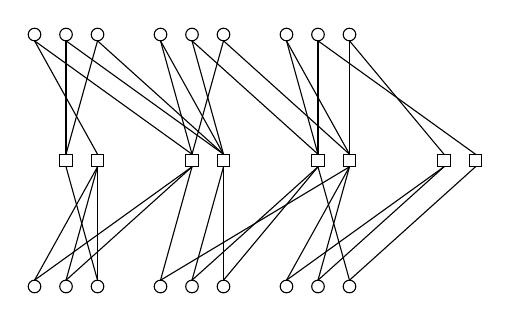
\begin{tikzpicture}[scale=0.8]

   \draw [black] (0,2) circle (0.1);  \draw [black] (0,-2) circle (0.1);
\draw [black] (0.6,0.1) rectangle (0.4,-0.1);  	\draw [black] (0.5,2) circle (0.1);  \draw [black] (0.5,-2) circle (0.1);
\draw [black] (1.1,0.1) rectangle (0.9,-0.1);     \draw [black] (1,2) circle (0.1);  \draw [black] (1,-2) circle (0.1);
  \draw (0,1.9) -- (2.5,0.1); \draw (0,1.9) -- (1,0.1);
\draw (0.5,1.9) -- (0.5,0.1); \draw (0.5,1.9) -- (3,0.1);
 \draw (1,1.9) -- (0.5,0.1); \draw (1,1.9) -- (3,0.1);

 \draw (0,-1.9) -- (2.5,-0.1); \draw (0,-1.9) -- (1,-0.1);
  \draw (0.5,-1.9) -- (2.5,-0.1); \draw (0.5,-1.9) -- (1,-0.1);
  \draw (1,-1.9) -- (0.5,-0.1); \draw (1,-1.9) -- (1,-0.1);

 \draw [black] (2,2) circle (0.1);  \draw [black] (2,-2) circle (0.1);
\draw [black] (2.6,0.1) rectangle (2.4,-0.1);  	\draw [black] (2.5,2) circle (0.1);  \draw [black] (2.5,-2) circle (0.1);
\draw [black] (3.1,0.1) rectangle (2.9,-0.1);  	\draw [black] (3,2) circle (0.1);  \draw [black] (3,-2) circle (0.1);
 \draw (2,1.9) -- (2.5,0.1); \draw (2,1.9) -- (3,0.1);
  \draw (2.5,1.9) -- (4.5,0.1); \draw (2.5,1.9) -- (3,0.1);
\draw (3,1.9) -- (2.5,0.1); \draw (3,1.9) -- (5,0.1);

 \draw (2,-1.9) -- (2.5,-0.1); \draw (2,-1.9) -- (5,-0.1);
 \draw (2.5,-1.9) -- (4.5,-0.1); \draw (2.5,-1.9) -- (3,-0.1);
  \draw (3,-1.9) -- (4.5,-0.1); \draw (3,-1.9) -- (3,-0.1);

\draw [black] (4,2) circle (0.1);  \draw [black] (4,-2) circle (0.1);
\draw [black] (4.6,0.1) rectangle (4.4,-0.1);      \draw [black] (4.5,2) circle (0.1);  \draw [black] (4.5,-2) circle (0.1);
\draw [black] (5.1,0.1) rectangle (4.9,-0.1);    \draw [black] (5,2) circle (0.1);  \draw [black] (5,-2) circle (0.1);
  \draw (4,1.9) -- (4.5,0.1); \draw (4,1.9) -- (5,0.1);
 \draw (4.5,1.9) -- (4.5,0.1); \draw (4.5,1.9) -- (7,0.1);
  \draw (5,1.9) -- (6.5,0.1); \draw (5,1.9) -- (5,0.1);

\draw (4,-1.9) -- (6.5,-0.1); \draw (4,-1.9) -- (5,-0.1);
 \draw (4.5,-1.9) -- (6.5,-0.1); \draw (4.5,-1.9) -- (5,-0.1);
 \draw (5,-1.9) -- (4.5,-0.1); \draw (5,-1.9) -- (7,-0.1);


\draw [black] (6.6,0.1) rectangle (6.4,-0.1);   %\draw [black] (13,2) circle (0.1);  \draw [black] (13,-2) circle (0.1);
\draw [black] (7.1,0.1) rectangle (6.9,-0.1);   %\draw [black] (14,2) circle (0.1);  \draw [black] (14,-2) circle (0.1);

 \end{tikzpicture}

%\end{document}
}
\caption{A $(2,6)$ SC-LDPC sub-graph of the ($3,6$) SC-LDPC graph shown in Fig.\ref{Basegraph}.}
\label{BaseGraph_sup}
\end{figure}

\subsection{Alternate construction}
In contrast to the previous construction where the check node degree remains constant over all the graphs in the sequence of nested codes, in this construction the variable node degree remains constant over all the graphs in the sequence of nested codes. Similar to the previous construction we explain for the case $r=2$.

Let the the required rates be $r_{1}, r_{2}$ , $0<r_{1}<r_{2}<1$. For small enough $\epsilon >0$, choose $d_{v}\geq 3$ such that there exists $d_{c}^{1},d_{c}^{2}\in \N$,
\begin{align}
		d_{c}^{2}=q d_{c}^{1}, q\in \N \hspace{0.3cm} \text{  and } \hspace{0.3cm}   1-\frac{d_{v}}{d_{c}^{i}}>r_{i}-\epsilon, i\in \{1,2\}.
\label{Eqn:DegreeConditions2}
\end{align}

In this construction of a nested pair of $\mc{C}_{1}\subseteq \mc{C}_{2}$ with SC-LDPC like structure, we first describe the construction of $\mc{C}_{2}$ and then the procedure of deriving the sub-code $\mc{C}_{1}$. The construction of $\mc{C}_{2}$ is identical to that of the $(d_{v},d_{c}^{2},L,w)$ SC-LDPC ensemble described in \cite{KudekarUrbanke11}. For sake of being self-contained we briefly describe the construction here. For details we refer the reader to  \cite{KudekarUrbanke11}.

Fix $M$ such that $\frac{Md_{v}}{d_{c}^{2}}\in \N$. We place $M$ variable nodes at positions $[1: L]$, $L\in\N$ and $\frac{Md_{v}}{d_{c}^{2}}$ check nodes at positions $[1 : L+w-1]$, where $w\in \N$ is the coupling width. From the variable node perspective we assign the edges such that each of the $d_{v}$ connections of a variable node at position $i$ is chosen uniformly at random from the range $[i : i+w-1]$. Ignoring the boundary effects, the above assignments are such that, for check nodes  at position $i$, the number of edges that come from variable nodes at position $i-j$, $j\in[0:w-1]$ is $\frac{Md_{v}}{w}$. In other words it is exactly $w^{\text{th}}$ fraction of the total number of edges at position $i$. We distribute these edges to $\frac{Md_{v}}{d_{c}^{2}}$ check nodes at position $i$ according to a permutation $\pi_{i}$ chosen uniformly at random from the set of permutations on $Md_{v}$ letters. With this we can also assume that each of the $d_{c}^{2}$ connections of a check node at position $i$ is independently chosen from the range $[i-w+1 : i]$. Until this point the construction is identical to the $(d_{v},d_{c}^{2},L,w)$ ensemble described in \cite{KudekarUrbanke11}, which we hereafter refer to as $(d_{v},d_{c}^{2},L,w)$ SC-LDPC ensemble. 

We will now describe the construction of a nested sub-code contained in a code from the above ensemble. Let a graph $\mc{G}_{2}$ be picked uniformly at random from the  $(d_{v},d_{c}^{2},L,w)$ SC-LDPC ensemble and let the binary code defined by this Tanner graph be $\mc{C}_{2}$. Consider a check node $C$ in $\mc{G}_{2}$ and
% and let's denote the set of bit nodes connected to the check node $c$ as $V_{c}$. 
replace the check node $C$ by check nodes $C_{1}, C_{2}, \ldots, C_{q}$ where each new check node $C_{i}$ has a degree $d_{c}^{1}$( Recall: $d_{c}^{2}=q d_{c}^{1},q\in \N$, by design). With an arbitrary ordering of the $d_{c}^{2}$ edges incident on $C$, distribute these edges to the new checks $C_{1}, C_{2}, \ldots, C_{q}$ according to a partition $\Pi_{C}$ picked uniformly at random from the set of all ``partitions of a set of $qd_{c}^{2}$ letters into $q$ subsets of equal size''. 
%the identity permutation of $d_{c}$ leters. permutation $P_{c}$ chosen uniformly at random from the set of all permutations on $d_{c}^{2}$ letters. 
Note that this operation, which we refer to as \textit{check-splitting}, does not alter the degree of  any variable node in the graph. By performing the \textit{check-splitting} operation on all the check nodes in $\mc{G}_{2}$, we derive a regular $(d_{v},d_{c}^{1})$ tanner graph. Let the derived graph be denoted $\mc{G}_{1}$ and let the binary code defined by $\mc{G}_{1}$ be $\mc{C}_{1}$.

\begin{lemma}\label{Lemma:NestedCodes}
$ \mc{C}_{1} \subseteq \mc{C}_{2}$.
\end{lemma}
\begin{proof}
Let $c$ be a check node in $\mc{G}_{2}$ and $\mbf{h}_{c}$ be the  corresponding parity-check vector (corresponding row in parity-check matrix). As each check node $c$ in $\mc{G}_{2}$ is replaced by check nodes $\{c_{1},\ldots , c_{q}\}$ in $\mc{G}_{1}$ let their corresponding parity check vectors be $\{\mbf{h}_{c_{1}},\ldots , \mbf{h}_{c_{q}}\}$. Clearly, from the construction,
\begin{align*}
\mbf{h}_{c}=\mbf{h}_{c_{1}}+\ldots +\mbf{h}_{c_{q}}.
\end{align*}
Consider $\mbf{x}\in\mc{C}_{1}$ and a check node $c\in \mc{G}_{2}$. As $\mbf{x}$ satisfies all the parity-check equations in $\mc{G}_{1}$, $\mbf{h}^{T}_{c_{i}}\cdot \mbf{x}\equiv 0 \mod 2, 1\leq i \leq q$.
\begin{align*}
\mbf{h}^{T}_{c}\cdot \mbf{x}&=\left[\mbf{h}^{T}_{c_{1}}+\ldots +\mbf{h}^{T}_{c_{q}}\right] \cdot \mbf{x}\\
												&\equiv 0 \mod 2. 
\end{align*}
The above implies $\mbf{h}^{T}_{c}\cdot \mbf{x}\equiv 0 \mod 2, \hspace{0.2cm} \forall c\in \mc{G}_{2}$ and hence $x\in \mc{C}_{2}$.
\end{proof}
One can obtain a sequence of nested linear codes $\mc{C}_1\subseteq\mc{C}_2\subseteq \ldots\subseteq\mc{C}_r$ by repeatedly performing the above operation, starting from $\mc{C}_{r}$. We observe that in this construction, unlike the previous construction, for any code $\mc{C}_{2}$ from the $(d_{v},d_{c}^{2},L,w)$ SC-LDPC ensemble, choice for deriving a sub-code is not unique. The non-uniqueness arises from the fact that for each check node `$c$' the number of choices for the partition $\Pi_{c}$ is not unique and any partition will result in a valid sub-code. We call the set of all $n$-tuples of codes $(\mc{C}_{1},\mc{C}_{2},\ldots,\mc{C}_{r})$, where $\mc{C}_{1}\subseteq \ldots\subseteq\mc{C}_{r}$ derived from the above construction as $(d_{v},d_{c}^{1},\ldots,d_{c}^{r})$ VC-SC-LDPC ensemble of nested codes. Here VC refers to \textit{variable-constant} since the variable degree remains constant across the nested sequence of codes. Here after whenever a nested chain of codes is referred to as SC-LDPC and no distinction between the constructions CU-SC-LDPC or VC-SC-LDPC is made, it is implied that the statement is valid for both the constructions. 

\begin{remark}\label{Rmk:EquivNestedConstr2}
Note that, given a code $\mc{C}_{2}$ from the $(d_{v},d_{c}^{2},L,w)$ SC-LDPC ensemble, deriving a sub-code $\mc{C}_{1}$ is equivalent to choosing a set of partitions: $\{\Pi_{c}: \tx{`}c\text{' is a check node in } \mc{C}_{2}\}$ uniformly at random. Therefore we can say that in this construction, for any choice of $\mc{C}_{2}$ there are equal number of choices for $\mc{C}_{1}$ from the $(d_{v},d_{c}^{1},L,w)$ SC-LDPC ensemble which are all equal likely.
\end{remark}


\begin{example}\label{Ex:ConstrD.2}
Under the VC-SC-LDPC construction, let's consider the same desired rates $r_{1}=0.5$ and $r_{2}=0.9$ as in Example~\ref{Ex:ConstrD.1}. By simple inspection one can see that the parameters $(d_{v},d_{c}^{1},d_{c}^{2})=(3,6,30)$ gives us nested VC-SC-LDPC codes of desired rates. Here we need to work with $(3,6)$ and $(3,30)$ SC-LDPC codes compared to $(15,30)$ and $(3,30)$ SC-LDPC codes in Example~\ref{Ex:ConstrD.1} based on the CU-SC-LDPC construction.
\end{example}

Since Construction-D works with generator matrices of nested linear codes, we have to obtain nested generator matrices from the proposed nested SC-LDPC codes. In the following lemma, we show the existence of such nested generator matrices for any set of nested binary linear codes.
\begin{lemma}\label{Lemma:NestedGeneratorMatrix}
    Given nested binary linear codes $\C_{1}\subseteq \mathcal{C}_{2}\subseteq\ldots \subseteq\mathcal{C}_{r}$ there exists nested generator matrices for these codes.
\end{lemma}
\begin{proof}
It suffices to consider the case having only two levels. For $\mathcal{C}_{1}$ there exists set of linearly independent binary vectors
$\mathbf{G}_{1}=\{\mathbf{g}_1,\mathbf{g}_2,\ldots, \mathbf{g}_{k_1}\}$ that span $\mathcal{C}_{1}$ where $k_{1}=$dim$(\mathcal{C}_{1})$.
Denote $\mathbf{Z}_{i}=\{\mathbf{G}_{1},\mathbf{g}_{k_{1}+1},\mathbf{g}_{k_{1}+2}, \ldots, \mathbf{g}_{k_{1}+i-1}\}$ and $Y_{i}=\mathcal{C}_{2}\setminus$
span$(\mathbf{Z}_{i})$ for $i=1,2, \ldots, k_{2}-k_{1}$. Note that for any $\mathbf{x}\in Y_{i}$, $\mathbf{x}$ is linearly independent with $\mathbf{Z}_{i}$ and hence
$\mathbf{Z}_{i+1}=\{\mathbf{Z}_{i},\mathbf{g}_{k_{1}+i}\}$ forms a linearly independent set where $\mathbf{g}_{k_{1}+i}=\mathbf{x}$. This recursive procedure gives us a basis $\mathbf{G}_{2}$ for $\mathcal{C}_{2}$. Thus the existence of the generator matrices for nested binary linear codes is shown.
\end{proof}
From Lemma~\ref{Lemma:NestedGeneratorMatrix}, given nested SC-LDPC codes $\mathcal{C}_{1}\subseteq \mathcal{C}_{2}\ldots \subseteq\mathcal{C}_{r}$, one can find a corresponding sequence of nested sets of generator vectors $\mathbf{G}_{1}\subseteq \mathbf{G}_{2} \subseteq \ldots \subseteq\mathbf{G}_{r}$ and hence one can use Construction-D described in \eqref{Eqn:ConstrD} with the proposed nested SC-LDPC codes. We refer to the lattice thus constructed as SC-LDPC lattice. Whenever required, we will make the distinction of the lattice being constructed from nested CU-SC-LDPC (or VC-SC-LDPC) sequence of codes by referring it to as a CU-SC-LDPC lattice (or VC-SC-LDPC lattice). 

\begin{remark}
For any code from the $(d_{v},d_{c},L,w)$ SC-LDPC ensemble, the design rate can be computed to be 
\begin{align}
\tx{R}(d_{v},d_{c},L,w)=1-\frac{d_{v}}{d_{c}}\frac{L+w-1}{L}.
\label{Eqn:DesignRate}
\end{align}
Similarly we define the design VNR of the proposed SC-LDPC lattices to be 
\begin{align*}
\alpha^{2}_{*}(\Lmb,\sigma^{2})=\frac{2^{2(r-\sum_{i=1}^{r}R_{i})}}{2\pi e\sigma^{2}}.
\end{align*}
where $R_{i}$ is the design rate of the $i^{\text{th}}$ code in the nested sequence of SC-LDPC codes. Although the design rate \eqref{Eqn:DesignRate} and the actual rate for any code from the ensemble are not necessarily equal, it is important to observe that the actual rate is atleast as large as the design rate, which gives the following inequality on the actual VNR of the SC-LDPC lattice,
\begin{align}
\alpha^{2}(\Lmb,\sigma^{2})\leq \alpha^{2}_{*}(\Lmb,\sigma^{2}).
\label{Eqn:VNRInequality}
\end{align}
%they are assumed to be equal (\textbf{Probably a reference for justification?}). 
\end{remark}


\subsection{Poltyrev-Goodness of the proposed lattices}
In this section we show the existence of a sequence of proposed lattices which is Poltyrev-good under BP decoding. In the following lemmas, we show that the proposed SC-LDPC codes (both the constructions) achieve the AMGN channel capacity. We then follow the argument by Forney \textit{et al.} described in Remark~\ref{Rmk:Forney_proof} to show the result.

\begin{lemma}\label{Lemma:DE_SCLDPC}
For a BMS channel with associated L-density $\mathbf{x}_{\text{BMS}}$\cite{richardson2008modern}, density evolution (DE) equation for a ($d_{v},d_{c},L,w$) CU-SC-LDPC ensemble is given by
\begin{align}
%x_{i}^{(l)}=\epsilon\left( 1-\frac{1}{w}\sum_{j=0}^{w-1}\left(1-\frac{1}{w}\sum_{k=0}^{w-1}x_{i+j-k}^{(l-1)}\right)^{d_{r}-1} \right)^{d_{l}-1},
\mathbf{x}_{i}^{(l)}\!=\!\mathbf{x}_{\text{BMS}}\!\circledast\!\bigg( 1-\frac{1}{w}\sum_{j=0}^{w-1}\!\Big(1-\frac{1}{w}\sum_{k=0}^{w-1}\mathbf{x}_{i+j-k}^{(l-1)}\Big)^{\boxast d_{c}-1} \bigg)^{\circledast d_{v}-1}
\label{Eqn:DE_SCLDPC}
\end{align}
where $\mathbf{x}_{i}^{(l)}$ is the average L-density of the message sent by a variable node at position $i$ in iteration $l$.
\end{lemma}
\begin{proof}
In the proposed CU-SC-LDPC ensemble, from the perspective of a variable node there are $d_{v}$ types of edges $\mc{E}_{1},\mc{E}_{2},\cdots,\mc{E}_{d_{v}}$. We denote edges of type $\mc{E}_{k}$ that originate from a variable node at position $i$ as $(i,\mc{T}_{k})$ and the L-density of the message emitted by variable nodes along such edge types as $\mathbf{x}_{ik}^{(l)}$ where $l$  denotes the iteration. But from the perspective of a check node of any type at position $i$, an edge is randomly connected to one of the variable nodes located at positions $\{i, i-1,... i-w+1\}$.	Hence all the edges connected to check nodes at a certain position are statistically identical and more importantly all check nodes at certain position are statistically identical. The average L-density of the message emitted by a check node at position $i$ in iteration $l$, denoted by $\mathbf{y}_{i}^{(l)}$, is given by
\begin{align}
\mathbf{y}_{i}^{(l)}=\left(\frac{1}{w}\sum_{j=0}^{w-1}\left(\frac{1}{d_{v}}\sum_{k=0}^{d_{v}}\mathbf{x}_{(i-j)k}^{(l-1)}\right)\right)^{\circledast d_{c}-1}
\label{Eqn:CheckNodeUpdate}
\end{align}
And a variable node update is given by
\begin{align}
\mathbf{x}_{ik}^{(l)}&=\mathbf{x}_{\text{BMS}}\boxast \left(\frac{1}{w}\sum_{j=0}^{w-1}\mathbf{y}_{i+j}^{(l)}\right)^{\boxast d_{v}-1}\label{Eqn:VariableNodeUpdate}\\
\mathbf{x}_{i}^{(l)}&=\frac{1}{d_{v}}\sum_{k=0}^{d_{v}}\mathbf{x}_{ik}^{(l)}\notag
\end{align}
where $\mathbf{x}_{i}^{(l)}$ is the average L-density of the log-likelihood ratio of variable nodes at position $i$.
Combining \eqref{Eqn:CheckNodeUpdate} and \eqref{Eqn:VariableNodeUpdate} and observing that the initialization
is $\mathbf{x}_{i}^{(1)}=\mathbf{x}_{i1}^{(1)}=\mathbf{x}_{i2}^{(1)}=\cdots=\mathbf{x}_{id_{v}}^{(1)}=\mathbf{x}_{\text{BMS}}$ completes the proof.
\end{proof}

Note that in \eqref{Eqn:DE_SCLDPC} we show that the DE equations for the proposed CU-SC-LDPC ensemble are identical to that of SC-LDPC ensemble proposed in \cite{KudekarUrbanke11,kudekaruniversal}.
\begin{remark}\label{Rmk:Same_DE}
In the VC-SC-LDPC construction of nested sequence of codes, a $(d_{v},d_{c},L,w)$ SC-LDPC ensemble is identical to the one in \cite{kudekaruniversal} and hence the DE equations in \eqref{Eqn:DE_SCLDPC} also hold valid for the $(d_{v},d_{c},L,w)$ SC-LDPC ensemble.
\end{remark}

\begin{lemma}\label{Lemma:BMSProof1}
For any $\delta$, $\epsilon>0$, there exists parameters $d_{c},d_{v},L,w$ such that the design rate $\tx{R}(d_{v},d_{c},L,w)>\tx{C}_{\text{AMGN}}(\sigma^{2})-\delta$ and a code $\mc{C}$ from the  $(d_{v},d_{c},L,w)$ CU-SC-LDPC  ensemble such that $\tx{P}_{\tx{b}}^{\text{BP}}(\mc{C},\sigma^{2})< \epsilon$, where $\tx{P}_{\tx{b}}^{\tx{BP}}(\mc{C},\sigma^{2})$ is the average bit error probability under BP decoding for $\mc{C}$ over AMGN channel with noise variance $\sigma^{2}$ and $\tx{C}_{\text{AMGN}}(\sigma^{2})$ is the corresponding Shannon capacity.
\end{lemma}
\begin{proof}
It has been proved in \cite{kudekaruniversal,kumar2014threshold} that over any BMS channel, under BP decoding, any system that satisfies the equation \eqref{Eqn:DE_SCLDPC} achieve the capacity as $d_{v},w,L \rightarrow \infty$ (with $\frac{d_{v}}{d_{c}}$ fixed), in that order. Hence if we show that the AMGN channel described in \eqref{Eqn:Mod2Channel} is indeed a BMS channel, then from Lemma~\ref{Lemma:DE_SCLDPC} it follows that there exist $d_{c},d_{v},L,w$ large enough such that the design rate $\tx{R}(d_{v},d_{c},L,w)>\tx{C}_{\text{AMGN}}-\epsilon$ and the bit error probability $\rightarrow 0$  as $M\rightarrow \infty$. It is clear to see that the AMGN channel has binary input and output lying in an interval of length $2$. Let the input alphabet to the channel be $\{0,1\}$ and without loss of generality let the $\mod 2$ operation produces a output lying in $[-0.5,  1.5]$. Then the conditional PDFs of $\mathbf{y}$ can be written as
\begin{align}
f(y|x=0)&=\frac{1}{\sqrt[]{2\pi e\sigma^{2}}}\sum_{j=-\infty}^{\infty}\exp\left[\frac{ -(y+2j)^{2}}{2\sigma^{2}}\right]\\
f(y|x=1)&=\frac{1}{\sqrt[]{2\pi e\sigma^{2}}}\sum_{j=-\infty}^{\infty}\exp\left[\frac{ -(y+2j-1)^{2}}{2\sigma^{2}}\right].
\end{align}
Therefore the PDFs of the output satisfy
\begin{align*}
f(y-0.5|1)=f(0.5-y|0) \hspace{10pt} \text{ for all } y\in [-0.5, 1.5].
\end{align*}
Thus, it belongs to the class of BMS channels.
\end{proof}

\begin{lemma}\label{Lemma:BMSProof2}
For any $\delta ,\epsilon>0$, there exists $d_{c},d_{v},L,w$ and code $\mc{C}$ from ($d_{c},d_{v},L,w$) SC-LDPC  ensemble such that the design rate $\tx{R}(d_{v},d_{c},L,w)>\tx{C}_{\text{AMGN}}(\sigma^{2})-\delta$ and $\tx{P}_{\tx{b}}^{\text{BP}}(\mc{C}_{i},\sigma^{2})< \epsilon$.

%For any $\epsilon>0$, there exists a sequence of codes, parameterized by $M$, from ($d_{c},d_{v},L,w$) SC-LDPC  ensemble such that the design rate $R(d_{v},d_{c},L,w)>C_{\text{AMGN}}-\epsilon$ and the bit error probability under BP decoding $\rightarrow 0$  as $M\rightarrow \infty$, where $C_{\text{AMGN}}$ is the Shannon capacity of the AMGN channel.
\end{lemma}
\begin{proof}
The proof in Lemma \ref{Lemma:BMSProof1} that AMGN channel is BMS and Remark~\ref{Rmk:Same_DE} gives us the required result.
\end{proof}

We have shown that there exists good codes from the ensembles of both the constructions, where by a `good code' we mean a code with the design rate arbitrarily close to the capacity of the AMGN channel and an arbitrarily small probability of error under BP decoding. But for using Construction-D and to be able to apply Forney's result we need to show existence of nested sequence of codes from the proposed constructions where each code in the sequence is a good code. We show this in the following theorems.

\begin{lemma}\label{Lemma:NestedGoodCodes1}
Given $r,\sigma^{2}$, for any $\epsilon>0$, there exists $d_{c},d_{v}^{1},\ldots, d_{v}^{r},L,w,$ and a nested sequence of codes $\mc{C}_{1}\subseteq \mc{C}_{2}\subseteq\ldots \subseteq\mc{C}_{r}$ from the $(d_{c},d_{v}^{1},\ldots,d_{v}^{r},L,w)$ CU-SC-LDPC ensemble such that 
\begin{align}
\tx{R}(d_{v}^{i},d_{c},L,w)&>\tx{C}_{\text{AMGN}}\left(\sigma^{2}_{i}\right)-5\epsilon, \text{ and} \label{Eqn:RateConditions1}\\
\tx{P}_{\tx{b}}^{\tx{BP}}\left(\mc{C}_{i},\sigma^{2}_{i}\right)&<\epsilon \hspace{0.5cm}\text{ for }1\leq i \leq r\label{Eqn:Error Prob1},
\end{align}
where $\sigma_{i}^{2}=\frac{\sigma^{2}}{2^{2(i-1)}}$ is the effective noise variance of the AMGN channel observed 	at the $i^{\text{th}}$ stage of multi-stage decoding.
%and $P_{b}^{BP}\left(\mc{C}_{i},\sigma_{i}\right)$ denotes the average bit error probability under BP decoding for $\mc{C}_{i}$ over AMGN channel of noise variance $\sigma_{i}^{2}$.
\end{lemma}

\begin{proof}
We will prove the result for the case $r=2$ i.e., the existence of a good nested pair of codes and for the cases $r>2$ the  proof extends naturally. Given $r=2$, for the given $\epsilon,\delta$ we choose $d_{c}$ large enough such that there exists parameters $d_{v}^{1},d_{v}^{2},L,w$ that satisfy \eqref{Eqn:RateConditions1} simultaneously for $i \in\{1,2\}$. For these parameters Lemma~\ref{Lemma:BMSProof1} guarantees us the existence of codes $\mc{C}_{i}\in\mc{E}_{i}\coleq (d_{c},d_{v}^{i},L,w)$ CU-SC-LDPC ensemble such that \eqref{Eqn:Error Prob1} is satisfied for $i\in\{1,2\}$.

It was not only shown in \cite{kudekaruniversal} that any system that satisfies \eqref{Eqn:DE_SCLDPC} is capacity-achieving  asymptotically in $d_{v},d_{c},w,L$ but also that almost all codes of sufficient length in the ensemble are good over a BMS channel. More precisely, it (\cite{kudekaruniversal} Corollary 43) states that for a given $\epsilon >0$, there exists $d_{v},d_{c}, L,w$ such that $\tx{R}(d_{v},d_{c},L,w)\geq \tx{C}_{\tx{AMGN}}(\sigma^{2})-5\epsilon$ and
\begin{align}
\lim_{n\rightarrow\infty}\mbb{E}_{\mc{C}(n)\in(d_{v},d_{c},L,w)}\left[ \ind_{\{\tx{P}_{\tx{b}}^{\tx{BP}}\left(\mc{C}(n),\sigma^{2}\right)\leq \epsilon\}}\right]=1,
\label{Corollary:AlmostGoodEnsemble}
\end{align}
where the average is over all codes $\mc{C}(n)$ of blocklength `$n$' from the $(d_{v},d_{c},L,w)$ SC-LDPC ensemble under uniform distribution. From Lemma~\ref{Lemma:DE_SCLDPC}, $(d_{v},d_{c},L,w)$ CU-SC-LDPC ensemble satisfies \eqref{Eqn:DE_SCLDPC} and hence \eqref{Corollary:AlmostGoodEnsemble} is valid for the $(d_{v}^{i},d_{c},L,w)$ CU-SC-LDPC ensembles, $i\in\{1,2\}$. Hence we can choose $n$ large enough such that 
\begin{align}
\mbb{E}_{\mc{C}_{i}(n)\in \mc{E}_{i}}\left[	 \ind_{\{\tx{P}_{\tx{b}}^{\tx{BP}}\left(\mc{C}_{i}(n),\sigma^{2}\right)\leq \epsilon\}}\right]\geq 1-\epsilon_{1},
\label{Eqn:Proof1.1}
\end{align}
for $i\in \{1,2\}$ where  the the average is over all codes of blocklength $n$ from $\mc{E}_{1}$.

 From Remark~\ref{Rmk:EquivNestedConstr1}, this construction is equivalent to first choosing $\mc{C}_{2}$ uniformly at random from $\mc{E}_{2}$ and then choosing $\mc{C}_{1}$ uniformly at random from the set $\mc{E}_{1}(\mc{C}_{2})\coleq \{\mc{C}_{1}:\mc{C}_{1}\in \mc{E}_{1},\mc{C}_{1}\subseteq \mc{C}_{2}\}$. From the fact that the set $\mc{E}_{1}(\mc{C}_{2})$ has same cardinality for all choices of $\mc{C}_{2}$ (see remark \ref{Rmk:EquivNestedConstr1}), we can deduce that the marginal distribution for $\mc{C}_{1}$ is uniform on $\mc{E}_{1}(\mc{C}_{2})$.\\
 For being concise we refer to code $\mc{C}_{i}\in\mc{E}_{i}$ as good if $\tx{P}_{\tx{b}}^{\text{BP}}(\mc{C}_{i},\sigma^{2})\leq \epsilon_{2}$ and bad if otherwise. Consider the probability of choosing a bad code for either levels,
 \begin{align*}
\tx{Pr}&\left[~ \mc{C}_{2}  \tx{ is bad  or } \mc{C}_{1} \tx{ is bad }\right] \\
&=\tx{Pr}\left[~\mc{C}_{2} \tx{ is bad } \right] +\tx{Pr}\left[~\mc{C}_{1} \tx{ is bad} \middle\vert \mc{C}_{1} \in \mc{E}_{1}(\mc{C}_{2}) \right] \\
&\leq \tx{Pr}\left[\mc{C}_{2} \tx{ is bad} \right] +\tx{Pr}\left[\mc{C}_{1} \tx{ is bad}\middle\vert \mc{C}_{1} \in \mc{E}_{1}\right] \\
&\leq 2\epsilon_{1}
 \end{align*}
 where the last inequality follows from%the uniform marginal distribution on $\mc{C}_{1}$ and 
 Eq. \eqref{Eqn:Proof1.1}. This not only gives us the existence of a good pair of nested codes arbitrarily close to capacity but also that almost all nested pairs from $(d_{c},d_{v}^{1},d_{v}^{2})$ CU-SC-LDPC ensemble are good.
\end{proof}

\begin{lemma}\label{Lemma:NestedGoodCodes2}
Given $r,\sigma^{2}$, for any $\epsilon>0$, there exists $d_{c},d_{v}^{1},\ldots, d_{v}^{r},L,w,$ and a nested sequence of codes $\mc{C}_{1}\subseteq \mc{C}_{2}\ldots \subseteq\mc{C}_{r}$ from the $(d_{v},d_{c}^{1},\ldots,d_{c}^{r},L,w)$ VC-SC-LDPC ensemble such that \eqref{Eqn:RateConditions1} and \eqref{Eqn:Error Prob1} are satisfied.
\end{lemma}
	\begin{proof}
In the proof of Lemma \ref{Lemma:NestedGoodCodes1}, using remark \ref{Rmk:Same_DE}, Lemma~\ref{Lemma:BMSProof2} and remark \ref{Rmk:EquivNestedConstr2}  instead of  Lemma~\ref{Lemma:DE_SCLDPC}, Lemma~\ref{Lemma:BMSProof1} and remark \ref{Rmk:EquivNestedConstr1} respectively gives us the required proof.	
\end{proof}

\begin{theorem}\label{Thm:Poltyrev_good1}
   For any $\epsilon,\delta>0$, there exists a CU-SC-LDPC lattice $\Lmb$ with $\alpha^2(\Lmb,\sigma^2)<1+\epsilon$ for which, under multistage BP decoding, the average probability of error $\tx{P}(\Lmb,\sigma^{2})<\delta$.
\end{theorem}
\begin{proof}
We first choose $r$ large enough such that 
\begin{equation}
\tx{P}\left(\Z_{2^{r}}^{n},\sigma_{r+1}\right)<\frac{\delta}{r+1},\notag
\end{equation}
where $\tx{P}\left(\Z_{2^{r}}^{n},\sigma_{r+1}\right)$ is the average error probability in decoding a point chosen uniformly at random from $\Z_{2^{r}}^{n}$ under minimum distance decoder. 
Then from Lemma~\ref{Lemma:NestedGoodCodes1}, there exists $(d_{c},d_{v}^{1},\ldots,d_{v}^{r})$ and nested sequence of codes $(\mc{C}_{1}, \mc{C}_{2}, \ldots,\mc{C}_{r})$ from the $(d_{c},d_{v}^{1},\ldots,d_{v}^{r})$ CU-SC-LDPC ensemble such that 
\begin{align}
\tx{R}(d_{v}^{i},d_{c},L,w)&>\tx{C}_{\text{AMGN}}\left(\sigma_{i}\right)-\epsilon_{1}, \text{ and} \\
\tx{P}_{\tx{b}}^{\tx{BP}}\left(\mc{C}_{i},\sigma_{i}\right)&<\epsilon_{2} \hspace{0.5cm}\text{ for }1\leq i \leq r.
\end{align}	
By union bound,  %Then for $n$ large enough we use the approximation ,(\textcolor{red}{This approximation is actually an upper bound for any n})
\begin{equation}\label{Eqn:Ineq-UncodedLevel}
\tx{P}^{\tx{BP}}(\mc{C}_{i},\sigma^{2}_{i})< n~\tx{P}_{\tx{b}}^{\tx{BP}}(\mc{C}_{i},\sigma^{2}_{i})
\end{equation}
 where $\tx{P}^{\tx{BP}}(\mc{C}_{i},\sigma^{2}_{i})$ is the corresponding block error probability. We then choose $\epsilon_{2}=\frac{\delta}{n(r+1)}$, use the union bound to bound the total error probability in decoding a lattice point which results in $\tx{P}(\Lmb,\sigma^{2})<\delta$. Recalling remark~\ref{Rmk:Forney_proof} and then the Eqn \eqref{Eqn:VNRInequality} bounding the actual VNR completes the proof.
\end{proof}

\begin{theorem}\label{Thm:Poltyrev_good2}
   For any $\epsilon,\delta>0$, there exists a VC-SC-LDPC lattice $\Lmb$ with $\alpha^2(\Lmb,\sigma^2)<1+\epsilon$ for which, under multistage BP decoding, the average probability of error $\tx{P}(\Lmb,\sigma^{2})<\delta$.
\end{theorem}
\begin{proof}
In the proof of Theorem \ref{Thm:Poltyrev_good1}, using Lemma~\ref{Lemma:NestedGoodCodes2} instead of Lemma~\ref{Lemma:NestedGoodCodes1} completes the proof. \end{proof}

\begin{remark}
Although lattices based on both the constructions have shown to be Poltyrev-good, both have their own pros and cons (advantages and disadvantages?). The parameters $(d_{c},d_{v}^{1},\ldots,d_{v}^{r})$ in the CU-SC-LDPC construction admit any set of natural numbers and thus give greater flexibility in constructing codes of desired rates at each level and thus provides the ability to match the capacity of the effective AMGN channel with a greater accuracy. But on the flip side this results in higher degree profiles, as explained in example~\ref{Ex:ConstrD.1}, and hence making the decoding more complex.  Whereas in the case of VC-SC-LDPC construction, the parameters only admit sets of the form $(d_{v},q_{1}d_{c},q_{2}d_{c},\ldots,q_{r}d_{c})$, $q_{i}\in\N$, which is not very flexible when it comes to  matching a given rate-tuple. But as we seen in examples~\ref{Ex:ConstrD.1} and~\ref{Ex:ConstrD.2}, in certain specific cases of desired rates, VC-SC-LDPC offers nested sequence of codes of considerably low complex degree profiles compared to the CU-SC-LDPC construction.
\end{remark}

\begin{remark}[Comparison with LDPC lattices]
    LDPC codes have been adopted as underlying codes for constructing lattices in \cite{sadeghi06} where the so-called LDPC lattices have been proposed and analyzed. Our SC-LDPC lattices differ from LDPC lattices in the following ways. Firstly, LDPC lattices are constructed based on Construction-D$^{\prime}$ \cite{BarnesSloane83} in contrast to Construction-D adopted here. Secondly, our decoding algorithm is a multistage BP decoding which only works over $\mbb{F}_2$, on the contrary, since constructed based on Construction-D$^{\prime}$, LDPC lattices have to consider BP algorithm on the joint Tanner graph \cite{Banihashemi01} (i.e., joint decoding). Last but not least, since there are no analytical evidence that LDPC codes under BP decoding would achieve capacity, LDPC lattices have not been shown Poltyrev-good to the best of our knowledge while for the proposed SC-LDPC lattices, Theorems~\ref{Thm:Poltyrev_good1} and~\ref{Thm:Poltyrev_good2} serves as constructive evidence.
\end{remark}


\subsection{Design and simulation results}
%In this subsection, we explain the design example of SC-LDPC lattices that approach the Poltyrev limit. Before we explain the design of Poltyrev-good SC-LDPC lattices, let's analyze the decoding error probability.

In this subsection, we explain the design of SC-LDPC lattices that approach the Poltyrev limit with examples. Before the design principles  let us analyze the decoding error probability.

Let the number of levels required be $r+1$, with $r$ coded levels using nested SC-LDPC codes and the last level being uncoded using the $\Z_{2^r}^{n}$ lattice. The design criteria depend mainly on the target error probability and the dimension of the lattice. For illustration let the  target block error probability be $\approx10^{-4}$ and the number of dimensions be $n=2 \times 10^{5}$.
As we use multistage decoding the average probability of decoding error $\tx{P}(\Lmb,\sigma^{2})$ can be union bounded by the sum of block error probabilities at individual levels. Assuming the constituent SC-LDPC code at each level is operating below the BP threshold\cite{richardson2008modern}, the average probability of decoding error of the lattice is dominated by the performance of the last (uncoded) level since the class of LDPC codes have a very sharply decaying error probability profiles below the BP threshold. Let's recall that  $\tx{P}(\Z_{2^r}^{n},\sigma^{2})$ is the block error probability for the last level. Similar to \eqref{Eqn:Ineq-UncodedLevel}, using union bound,
\begin{align}
\tx{P}(\Z_{2^r}^{n},\sigma_{\tx{r+1}}^{2})&\leq n\tx{P}(\Z_{2^r},\sigma^{2})=n\left(2Q\left(\frac{0.5}{\sigma_{r+1}}\right)	\right).
\label{Eqn:ZLatticeProb}
\end{align}

\begin{figure}[!ht]
\centering
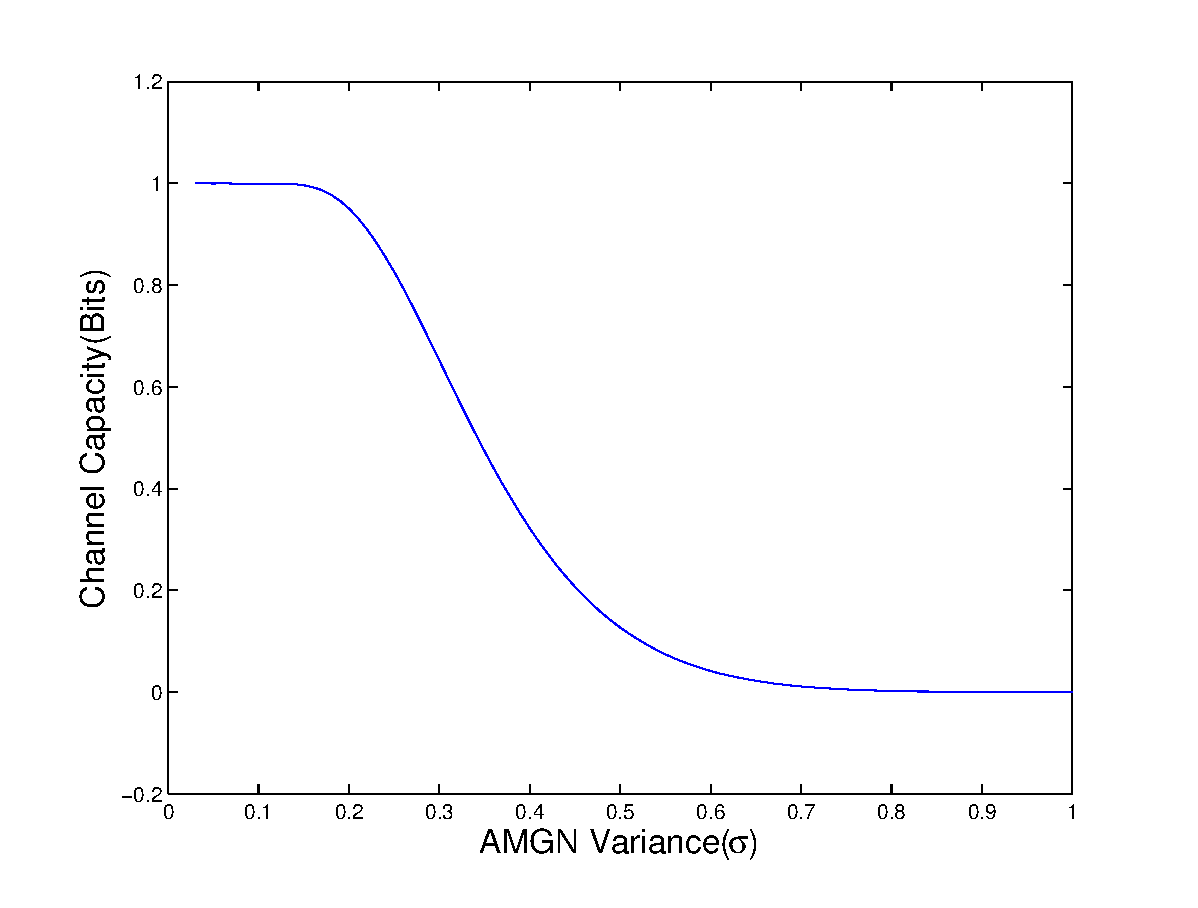
\includegraphics[width=0.9\textwidth]{./figures/SCLDPC_lattices/Cap_integer_coset_lattice.eps}
\caption{Channel capacity of the additive mod-2 Gaussian noise channel}
\label{Fig:AMGNCapacity}
\end{figure}

Plugging in the values of $n$ and the target error probability in \eqref{Eqn:ZLatticeProb} gives us $\sigma_{r+1}= 0.0804$. Now moving to the next level i.e., level $r$, $\sigma_{r}=2\sigma_{r+1}=0.1608$. The capacity of the effective AMGN channel observed in this level of the multi-stage decoding is $\tx{C}_{\tx{AMGN}}(\sigma^{2}_{r})=0.9923$, see Fig. \ref{Fig:AMGNCapacity}. For the details on computing the capacity of the AMGN channel see \cite{forney2000}.  Similarly proceeding, $\sigma_{r-1}=2\sigma_{r}=0.3217$, $\tx{C}_{\tx{AMGN}}(\sigma^{2}_{r-1})=0.5726$, $\sigma_{r-2}=2\sigma_{r-1}=0.6434$, $\tx{C}_{\tx{AMGN}}(\sigma^{2}_{r-2})=0.0242$. Observe that the capacity for level $r-2$ is almost zero which renders coding for this level unnecessary albeit at the cost of a very small increase in VNR (due to the rate loss) of $0.145$dB $(=20\log_{10}2^{0.0242})$. Hence $r=2$ i.e., two coded levels suffice. We use ($30,14,3$) CU-SC-LDPC ensemble with $L=32, w=4$ for the first two levels and $\Z_{4}^{n}$ lattice for the last level which results in nested SC-LDPC codes of rates $0.5333$ and $0.9$ ($0.49$ and $0.89$ including rate-loss due to boundary effects of coupling) matching closely the capacities of first two levels i.e. $0.5726$ and $0.99$.
\begin{table}
\centering
\begin{tabular}{c c c c c c}
\hline  \hline
$(d_{c},d_{v}^{1},d_{v}^{2})$ &(L,w)& $\sigma_{\text{max}}$ &$\text{VNR}^{*}$(dB) &$\text{VNR}_{\text{rate-loss}}$(dB)\\
\hline
(30,14,3) & (32,4) & 0.3184 & 1.14 & 1.347\\
(60, 27, 3)& (64, 9)  &  0.3203 & 0.57 & 0.951 \\
(60, 26, 3)& (72, 12) & 0.3200 &0.482 & 0.927\\
(60, 42, 3)& (72, 12) & 0.3975 & 0.203 &1.02\\
%(30,14,3) & (32,4) & 0.3184 &0.2184 &1.14dB&1.347dB\\
%(60, 27, 3)& (64, 9)  &  0.3203 & 0.1953 &0.57dB&0.951\\
%(60, 26, 3)& (72, 12) & 0.3200 & 0.1953 &0.482dB&0.927dB\\
%(60, 42, 3)& (72, 12) & 0.3975 & 0.1953 &0.203dB&---
%(60,42,3)&(72,12)&0.3975&0.1953&0.203dB\footnote{Target Bit Error Probability of $10^{-6}$}&---
\end{tabular}
\caption{Density evolution (DE) thresholds for SC-LDPC lattice ensembles under BP decoding for various degree profiles. The gap from the respective Poltyrev limits, computed without considering rate loss from termination, are also given.}
\label{Table:Thresholds}
\end{table}

\subsubsection*{Simulation results}
Due to symmetry in the lattice the all-zero lattice point is assumed to be transmitted. Instead of plotting the symbol error rate, we focus on determining the thresholds of the resulting lattice under BP decoding. We estimate the BP threshold from simulations by determining the maximum noise variance for which no codeword errors are observed, at each coded level, in simulation of 10 consecutive codewords each of length $2\times 10^{5}$. We calculate the maximum variance $\sigma_{\tx{max}}^{2}$ for which all the levels of the lattice can be decoded given by $\sigma_{\text{max}}=\min(\sigma_{1}^{\text{BP}},2\sigma_{2}^{\text{BP}},\sigma_{3})$, where $\sigma_{1}^{\text{BP}}$ and $\sigma_{2}^{\text{BP}}$ are the respective BP thresholds for the two SC-LDPC codes and $\sigma_{3}^{2}$ is the noise variance at which the uncoded level achieves the target error probability. The VNR threshold is then calculated for the given rates and $\sigma_{\text{max}}$. Thus obtained BP thresholds $\sigma_{1}^{\text{BP}}$, $\sigma_{2}^{\text{BP}}$ for the above codes are $0.3142$ and $0.2161$ respectively which results in a VNR of $1.14$dB ($1.46$dB with rate loss due to termination). The DE predicted values are $0.3184$ and $0.21836$. We observe that the BP thresholds are very close to DE thresholds. i.e., the parameters are large enough to assume that the BP thresholds can be approximated by DE thresholds. Therefore it is reasonable to calculate the VNR thresholds using the DE thresholds. For various SC-LDPC ensembles Table. \ref{Table:Thresholds} gives us the VNR thresholds i.e., the VNRs achievable for respective target error probabilities which are computed using the DE thresholds. Note that the Poltyrev limit is zero dB, thus making the VNR threshold and the gap from Poltyrev limit equivalent. The gap to the Poltyrev limit is primarily due to the fact that there is a mismatch between the capacity of the equivalent channel and the rates that are obtainable for the proposed CU-SC-LDPC ensemble.  

In the above design, if we target a error probability per dimension of $10^{-6}$  instead, that gives us $\sigma_{r+1}= 0.0999$, capacities for the subsequent levels $\tx{C}_{\tx{AMGN}}(\sigma^{2}_{r})=0.9507$, $\tx{C}_{\tx{AMGN}}(\sigma^{2}_{r-1})=0.3223$ and $\tx{C}_{\tx{AMGN}}(\sigma^{2}_{r-2})=0.0024$. Pair of nested codes from $(60,42,3)$ CU-SC-LDPC ensemble gives us rates $0.3$ and $0.95$ resulting in better matching of the rates (negligible rate loss). The resulting DE thresholds are within $0.203$dB from Poltyrev limit. This is reported in the last row in the table. [Couple of lines - Broadly justifying the VC-SC-LDPC construction] Observe that for these parameters we can use a $(60,4,3)$ VC-SC-LDPC ensemble with the same parameters of $(L=72,w=12)$ gives us codes of rates $0.25$ and $0.95$. Although this results in a slight VNR-loss due to the relatively poor mismatching of rates, in this case BP decoding is carried out on a $(3,4)$ Tanner graph instead of a $(42,60)$ which considerably reduces the complexity of decoding.

\section{Application - Interference Channel}
\subsection{Problem statement}
We consider the 3 user Gaussian interference channel (IC) consisting of 3 transmitters, 3 receivers, and 3 independent messages originally considered in \cite{sridharan2008capacity}, where message $W_{j}$ originates at transmitter $j$ and is intended for receiver $j$, $\forall j\in \mc{J}\defeq\{1,2,3\}$. The output observed at the receiver $j$ is given by
\begin{align}\label{SymmInterfChannel}
    \mathbf{y}_{j}=\mathbf{x}_{j}+ \sum^{3}_{k=1,k\neq j}h_{jk}\mathbf{x}_{k}+\mathbf{z}_{j}, \hspace{10pt} \forall j\in \mc{J}
\end{align}
where $\mathbf{x}_{j}$ is the transmitted signal at $j^{\text{th}}$ transmitter, $h_{jk}$ are the channel parameters for the cross links, and $\mathbf{z}_{j}\sim\mc{N}(\mathbf{0},\sigma^{2}\cdot \mathbf{I})$ is the AWGN noise. If the channel parameters for all the cross links are equal we refer to such model as symmetric IC. The channel input signals are subjected to the power constraint
$\frac{1}{n}\sum_{i=1}^{n}E\left[\|\mathbf{x}_{j}\|^2\right]\leq P$.

For a $2$-user symmetric Gaussian interference channel (IC) it was shown in \cite{carleial1978interference} that, in the very strong interference regime, the capacity region for the IC is as if there is no interference at all. For this symmetric model, a simple extension of the very strong interference condition for the 2 user IC %\cite{carleial1978interference}
to the 3 user one is given by \cite{sridharan2008capacity}
\begin{align}
\beta^{2}\geq \frac{\left((1+P)^{2}-1\right)\left(1+P\right)}{2P}.
\label{Eqn:StrongInterfCondition1}
\end{align}

Sridharan \textit{et al.} in \cite{sridharan2008capacity} introduced the idea of lattice alignment where each user uses a lattice code and each receiver first decodes the total interference (aligned due to lattice structure) observed and then decodes the desired message. For this case, they derived a tighter condition on $\beta$ in order for the interference to be decoded first. This is based on lattice coding, independent of the number of users, and is given by
\begin{align}
\beta^{2}(\sigma)\geq \beta^{*^{2}}(\sigma)\defeq\frac{(P+\sigma^{2})^{2}}{P\sigma^{2}}
\label{Eqn:StrongInterfCondition2}
\end{align}
If \eqref{Eqn:StrongInterfCondition2} is satisfied, each user can achieve a capacity of $\frac{1}{2}\log(1+\frac{P}{\sigma^{2}})$ \cite{sridharan2008capacity}. Equivalently, for a given rate $R$, maximum noise variance under which the rate can be achieved is given by
\begin{align}
\sigma^{2}_{\text{max}}=\frac{P}{2^{2R}-1}.
\label{Eqn:SigmaShannon}
\end{align}

\subsection{Applying the proposed lattices}
Encouraged by the Poltyrev-limit achieving property of the proposed lattice ensembles under BP decoding, we use SC-LDPC lattice codes for the symmetric Gaussian IC in the very strong interference region. Let $\Lmb_{SC}$ be the SC-LDPC lattice defined in \eqref{Eqn:ConstrD} with $r=2$.
% and a code from $(30,15,5)$ CU-SC-LDPC ensemble is used for the two levels.
We define the SC-LDPC lattice code $\mc{C}_{SCL}$ based on $\Lmb_{SC}$ using hypercube shaping:
\begin{align}
\mc{C}_{SCL}=\left\lbrace \mathbf{\lmb} \mod \Z_{4}^{n}: \mathbf{\lmb} \in \Lmb \right\rbrace
\end{align}
where $n$ is the dimension of $\Lmb_{SC}$. Let codeword $\mathbf{c}_{j}\in\mc{C}_{SCL}$ at transmitter $j$ be
\begin{align}
\mathbf{c}_{j}&= \sum_{i=1}^{k_{1}}\alpha_{ji}\mathbf{g}_i+2\sum_{i=1}^{k_{2}}\beta_{ji}\mathbf{g}_i \mod \Z_{4}^{n}\hspace{15pt} \alpha_{ji},\beta_{ji}\in \{0,1\}\\
\label{Eqn:SICCodeword}
&= \sum_{i=1}^{k_{1}}\alpha_{ji}\mathbf{g}_i+2\sum_{i=1}^{k_{2}}\beta_{ji}\mathbf{g}_i -4\mathbf{k}_{j}, \ \mbox{for some} \ \mathbf{k}_{j}\in\Z^{n}
\end{align}
where "$+$" denotes addition in $\R^{n}$. Each codeword $\mathbf{c}_{j}\in\mc{C}_{SCL}\subset\{0,1,2,3\}^{n}$ is modulated to $\mathbf{\tilde{x}}_{j}\defeq 1.5^{n}-\mathbf{c}_{j}$ such that $\mathbf{\tilde{x}}_{j}\in\mc{A}\defeq\{-1.5,-0.5,+0.5,+1.5\}^{n}$. At transmitter $j$, a dither vector $\mathbf{d}_{j}$ uniformly distributed among $\mc{B}\defeq [-2,2)$ is added to obtain the transmitted signal $\mathbf{x}_j$ given by
\begin{align}
\mathbf{x}_{j}=\mathbf{\tilde{x}}_{j}+\mathbf{d}_{j} \mod \Z_{4}^{n},
\label{Eqn:SICdither}
\end{align}
where the mod operation is over $\mc{B}$ instead of $[0,4)$. The dither vector achieves the purpose of randomizing the interference and helps in treating the undesired components of the received signal as additive uncorrelated noise. It can be seen that $\mathbf{x}_{j}$ is uniformly distributed over $\mc{B}$ and the average power of the transmitted signal at each transmitter is $1.33$.

\begin{figure*}[t]
\centering
\resizebox{0.8\textwidth}{!}{
%\begin{document}
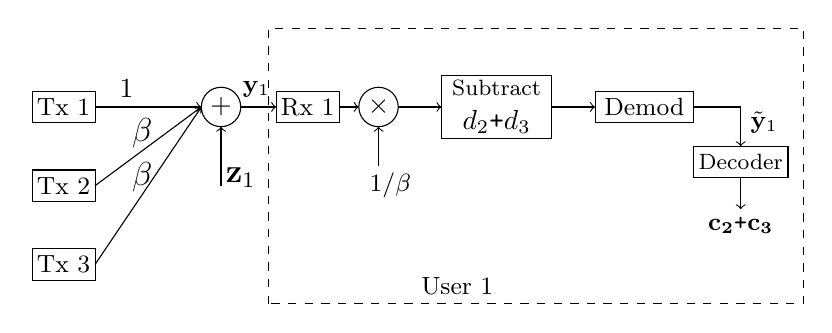
\begin{tikzpicture}
\def\fsize{\small}
%3 Users
\draw[black] (0.4,0.2) rectangle (-0.4,-0.2); \node at (0,0) {\fsize Tx 1};
\draw[black] (0.4,-0.8) rectangle (-0.4,-1.2); \node at (0,-1) {\fsize Tx 2};
\draw[black] (0.4,-1.8) rectangle (-0.4,-2.2); \node at (0,-2) {\fsize Tx 3};

%Oblique lines to Plus block
\draw [->] (0.4,0) -- (1.75,0); \node [above] at (0.8,0) {1};
\draw [->] (0.4,-1) -- (1.75,0); \node [above] at (1,-0.65) {\large $\beta$};
\draw [->] (0.4,-2) -- (1.75,0); \node [above] at (1,-1.2) {\large $\beta$};


%From + end to Rx1 end
\draw[black] (2,0) circle (0.25); \node at (2,0) {+};
\draw [->] (2,-1) -- (2,-0.25);\node at (2.25,-0.9) {\large $\mathbf{z}_{1}$};

%Receiver 1 block
\draw[black] (2.7,-0.2) rectangle (3.5,0.2); \node at (3.1,0) {\fsize Rx 1};
\draw [->] (2.25,0) -- (2.7,0);\node[above] at (2.45,0) {\fsize $\mathbf{y}_{1}$};

%From Rx1 end to 1/beta multiplicator end
\draw[black] (4,0) circle (0.25); \node at (4,0) {$\times$};
\draw [->] (4,-0.75) -- (4,-0.25);\node at (4.15,-1) {\fsize $1/\beta$};
\draw [->] (3.5,0) -- (3.75,0);

\draw[black] (4.8,0.4) rectangle (6.2,-0.4) node[pos=0.5,align=center] {\footnotesize Subtract\\ $d_{2}\texttt{+}d_{3}$}; 
%\node[text width=1.2,align=left] at (5.05,0) {\fsize Subtract  \\ $d_{2}\texttt{+}d_{3}$};
\draw [->] (4.25,0) -- (4.8,0);

% Input to the Demod
\draw[black] (6.75,0.2) rectangle (8,-0.2) node[pos=0.5,align=center] {\small Demod};
\draw [->] (6.2,0) -- (6.75,0);

%Input to Decoder
\draw [->](8,0) -- (8.6,0) -- (8.6,-0.5);
\node[right] at (8.6,-0.2) {\fsize $\tilde{\mathbf{y}}_{1}$};
\draw[black] (8,-0.9) rectangle (9.2,-0.5) node[pos=0.5,align=center]  {\footnotesize Decoder}; 

%Overview dashed rectangle
\draw [->] (8.6,-0.9) -- (8.6,-1.3);  \node at (8.6,-1.5){\fsize $\mathbf{c_{2}}\texttt{+}\mathbf{c_{3}}$};
\draw [dashed] (2.6,-2.5) rectangle (9.4,1);\node [above] at (5,-2.5) {\fsize User 1};

 \end{tikzpicture}
%\end{document} 
}
\caption{System flow for the 3-user Symmetric Gaussian Interference channel at receiver 1.}
\label{Fig:SIC_decoder}
\end{figure*}

\subsection{Decoding}
Before looking at the general case let us consider the symmetric Gaussian IC i.e $h_{12}=h_{13}$. Without loss of generality let us consider receiver 1. The system schematic from the perspective of receiver 1 is given in Fig.~\ref{Fig:SIC_decoder}. The input to the multistage decoder at receiver 1 is given by
\begin{align*}
\tilde{\mathbf{y}}_{1} &\defeq \frac{\mathbf{y}_{1}}{h_{12}}-\mathbf{d}_{2}-\mathbf{d}_{3}+1.5^{n}+1.5^{n}\\%\mod \Z_{4}^{n} \\
&=\mathbf{c}_{2}+\mathbf{c}_{3}+\frac{1}{h_{12}}\left(\mathbf{x}_{1}+\mathbf{z}_{1}\right).
\end{align*}
Note that $\mathbf{c}_{2},\mathbf{c}_{3}\in\mc{C}_{SCL}\subset\Lmb$ and hence $\mathbf{c}_{2}+\mathbf{c}_{3}\in \Lmb$.
\begin{align*}
\mathbf{c}_{2}+\mathbf{c}_{3}&=\sum_{i=1}^{k_{1}}\left(\alpha_{2i}+\alpha_{3i}\right)\mathbf{g}_i+2\sum_{i=1}^{k_{2}}\left(\beta_{2i}+\beta_{3i}\right)\mathbf{g}_i +4\mathbf{k}_{2}+4\mathbf{k}_{3}\\
&=\sum_{i=1}^{k_{1}}\left(\alpha_{2i}\oplus\alpha_{3i}\right)\mathbf{g}_i+2\sum_{i=1}^{k_{2}}\left(c_{1i}\oplus\beta_{2i}\oplus\beta_{3i}\right)\mathbf{g}_i +4\mathbf{k}_{23}
\end{align*}
where $c_{1i}=0.5\left(\alpha_{2i}+\alpha_{3i}-\alpha_{2i}\oplus\alpha_{3i}\right)$, $c_{2i}=0.5\left(c_{1i}+\beta_{2i}+\beta_{3i}-c_{1i}\oplus\beta_{2i}\oplus\beta_{3i}\right)$ are carryovers from first and second levels respectively and
 $\mathbf{k}_{23}=\mathbf{k}_{2}+\mathbf{k}_{3}+\sum_{1}^{k_{2}}c_{2i}\mathbf{g}_{i}\in\Z^{n}$. The key here is that  $c_{1i}, c_{2i} \in \{0,1\}$ which lets us apply multi-stage BP decoding. Using multi-stage decoder described in Section \ref{Sec:SCLDPC}, one can directly decode the lattice point $\mathbf{x}_{2}+\mathbf{x}_{3}$(interference), subtract it and decode the desired signal.

The decoding scheme above extends to the case when one channel gain is an integer multiple of the other. For example, let $h_{13}=Kh_{12}$
where $K=\sum_{0}^{l-1}a_{i}2^{i}\in \Z, a_{i}\in\{0,1\}$. In this case, input to the multi-stage decoder is
\begin{align*}
\tilde{\mathbf{y}}_{1} &\defeq \frac{\mathbf{y}_{1}}{h_{12}}-\mathbf{d}_{2}-K\mathbf{d}_{3}+1.5^{n}+K1.5^{n}\\
&=\mathbf{c}_{2}+K\mathbf{c}_{3}+\frac{1}{h_{12}}\left(\mathbf{x}_{1}+\mathbf{z}_{1}\right).
\end{align*}
where $\mathbf{c}_{2}+K\mathbf{c}_{3}$ is a lattice point and is given by
\begin{align*}
%\mathbf{c}_{2}+K\mathbf{c}_{3}=
\sum_{i=1}^{k_{1}}\left(\alpha_{2i}\oplus a_{0}\alpha_{3i}\right)\mathbf{g}_i+2\sum_{i=1}^{k_{2}}\left(c_{1i}\oplus\beta_{2i}\oplus a_{0}\beta_{3i}\oplus a_{1}\alpha_{3}\right)\mathbf{g}_i+4\mathbf{k}
\end{align*}
for some $\mathbf{k}\in\Z^{n}$.


\subsection{Simulation results for symmetric IC}
\label{subsec:SCLDPC_IC_results}
In this section we present simulation results for the symmetric Gaussian IC and compare them with the bounds given in \cite{sridharan2008capacity}. We choose a pair of nested codes from the $(30,18,3)$ CU-SC-LDPC ensemble with spatial-coupling parameters $(L,w)=(32,4)$. We fix $\sigma=\sigma_{\text{max}}$ (such that in absence of interference, desired signal can be decoded successfully) and we analyze the bit error probability in decoding the interference versus the channel gain $\beta$. We observe that within $0.396$dB of the very strong interference regime given by \eqref{Eqn:StrongInterfCondition2} we are able to decode the interference with a bit error probability of less than $10^{-6}$. Note that the main bottle neck in error performance in decoding the interference is the last i.e., the uncoded level whereas in decoding the desired signal (after the interference is decoded and subtracted), within $\sigma_{\text{max}}$, arbitrarily small error rates can be achieved since no uncoded level needs to be decoded.

%On a single user AWGN channel i.e, after the interference is subtracted, the DE threshold for this code for the given parameters is computed to be $\sigma_{\text{max}}=0.3351$ whereas asymptotically the maximum achievable variance is $\sigma_{\text{AMGN}}=0.3728$. The Shannon capacity from \eqref{Eqn:SigmaShannon} is given by $\sigma_{\text{Sh}}=0.4969$ which is equivalent to a gap of $2.5$dB.

In Fig.~\ref{Fig:ShapingLoss}, we plot the achievable rate as a function of $P/\sigma^2$ for the desired user for $r=4$. It can be seen that the achievable rate with the lattice code has a gap of roughly 1.53~dB from the corresponding Shannon limit at high rates. This is the shaping loss due to hypercube shaping.  The DE thresholds with the proposed SC-LDPC codes is also shown in the plot and it can be seen that the DE thresholds are very close to the achievable rates.
%
%We also observe that as the number of levels increase this gap converges to $1.53$dB which corresponds to the loss due to the sub-optimal hypercube shaping. For a 4-level binary lattice code with hypercube shaping corresponding gap between shannon capacity and the sum-capacity of 4 levels is plotted  in Fig. \ref{Fig:ShapingLoss}. One can also observe that the sum-capacity can be very closely achieved with a SC-LDPC lattice code of maximum check node degree 60.
%Thus we claim that with optimal shaping strategies the capacity of the $K$-user symmetric Gaussian IC \cite{sridharan2008capacity} in the very strong interference channel can be achieved.

\begin{figure}
\centering
\setlength\figureheight{0.7\textwidth}
\setlength\figurewidth{0.85\columnwidth}
\begin{tikzpicture}
\def\fsize{\normalsize}
\begin{axis}[
width=\figurewidth,
height=\figureheight,
scale only axis,
xmin=4,
xmax=30,
xlabel={$\text{P/}\sigma{}^{\text{2}}\text{dB}$},
ymin=0,
ymax=5,
legend style={at={(0,1)},anchor=north west,draw=black,fill=white,legend cell align=left}
]
\addplot [color=red,solid,line width=1.5pt]
table[row sep=crcr]{
1 0.587818317346194\\
3 0.791341177455778\\
5 1.0286866043034\\
7 1.29390718678102\\
9 1.58040221195651\\
11 1.88219718352143\\
13 2.19452948368152\\
15 2.51390383667526\\
17 2.83788995090244\\
19 3.16485622972095\\
21 3.49373172947796\\
23 3.8238235812452\\
25 4.1546876206064\\
27 4.48604077166048\\
29 4.81770328916082\\
31 5.14956130632863\\
33 5.48154279616551\\
35 5.81360224010802\\
};
\addlegendentry{Shannon Capacity};

\addplot [color=blue,solid,line width=2.0pt]
table[row sep=crcr]{
1 0.108452421861326\\
3 0.30023434461803\\
5 0.583744051972549\\
7 0.908016893863155\\
9 1.23986729393466\\
11 1.57212348172311\\
13 1.90441001540582\\
15 2.23669080702334\\
17 2.56895109146972\\
19 2.90120263165125\\
21 3.23173038940203\\
23 3.54445589072375\\
25 3.7941222586385\\
27 3.93912155348957\\
29 3.99069691963094\\
31 3.99949543839257\\
33 3.99999469407798\\
35 3.99999999597798\\
};
\addlegendentry{Sum Capacity of 4-level Construction-D Lattice Code};

\addplot [color=black,mark size=3.0pt,only marks,mark=square,mark options={solid}]
table[row sep=crcr]{
21.4693 3.15\\ % 18.91 3.1501 
22.3844 3.2667\\  %19.621 3.2668 . The commented out values are the snr values at which the shannon capacity is equal
23.1876 3.4167\\  %20.532 3.4166 	   to the DE of the optimal degree profiles of the 4 level SCLDPC lattice code.
15.4486951388326 2.2\\
16.3638449500461 2.3167\\
17.1669877129645 2.4667\\
};
\addlegendentry{DE thresholds for 4-level SC-LDPC Lattice Codes};

\addplot [color=black,mark size=2.9pt,only marks,mark=asterisk,mark options={solid}]
table[row sep=crcr]{
23.2798476914952 3.41666666666667\\
22.4669998480458 3.26666666666667\\
16.3950035382421 2.31666666666667\\
17.2078513816915 2.46666666666667\\
};
\addlegendentry{BP thresholds for 4-level SC-LDPC Lattice Codes};


\draw[<->] (axis cs:18.91,3.1501 ) -- (axis cs:21.469, 3.15);
\draw[->] (axis cs:19.6,3.12) to [out=285,in=175] (axis cs:22,2.6);
%\node[font=\scriptsize] at (axis cs:14,3.6){1.57dB};
\node[font=\fsize] at (axis cs:24,2.6){2.559dB};

	\end{axis}
\end{tikzpicture}%
\caption{The gap between the Shannon capacity and the achievable sum-rate of a 4-level Construction-D lattice code(hypercube shaping) under multi-stage decoding. The DE thresholds, along with comparison with BP thresholds for $n=2\times10^5$, for various SC-LDPC lattice codes with a maximum check node degree of $60$ are also given.}	
\label{Fig:ShapingLoss}	
\end{figure}

%\section{Application - Bi-Directional Relay Channel}
%\subsection{Problem Statement}
%We consider the Bi-Directional Relay channel where two users try to communicate with each other with the help of a relay node acting as an intermediate. Objective is to design coding schemes at both the users and forwarding scheme at the relay such that at each user the message intended to be transmitted by the other user can be decoded, given the availability of the noise corrupted forwarded signal from the relay.
%The problem can be very simply described by these three equations: 
%\begin{align*}
%y_{R}=a x_{1}+b x_{2}+z \\
%y_{1}=x_{F}+z_{1} \\
%y_{2}=x_{F}+z_{2} 
%\end{align*}
% are received signals at Relay, and Users 1 and 2 respectively and $x_{F}$ is the signal forwarded by the relay and is a function of the  forwarding scheme we use. For simplicity let's assume that $a,b\in \Z$.
%
%\subsection{Proposed Scheme}
%We define a code (finite constellation) from the Poltyrev-good SC-LDPC lattice as follows:
%\begin{equation}
%\mc{C}\defeq \Lmb_{C}\cap \Z_{5}^{N}
%\end{equation}
%Rate of hence defined code will be $\log_{2}(2^{r_{1}+r_{2}}\frac{5}{4})=r_{1}+r_{2}+\log_{2}(\frac{5}{4})$ bits/dim. User $i$ picks a codeword $x_{i}\in\mc{C}$ uniformly and transmits. The received signal at relay is:
%\begin{align*}
%y_{R}=a x_{1}+b x_{2} +z
%\end{align*}
%The additive group structure of the lattice and the fact that $x_{1},x_{2}\in \Lmb_{C}$ gives us $a x_{1}+b x_{2}\in \Lmb_{C}$. Using the multi-stage decoding described previously we decode the lattice point $a x_{1} + b x_{2}\in \Lmb_{C}$. Note that in the decoder we need to do the euclidean decoder in the last stage too since not just the corresponding coset of $a x_{1}+b x_{2}$ suffices but we need the actual lattice point.

%For the forwarding part, we compute 
%\begin{align}
%x_{F}=a x_{1} +b x_{2} \mod 5\Z^{N}.
%\end{align}
%Note that since $5\Z^{N}\not \subset \Lmb_{C}$, $x_{F}\in \Lmb_{C}$ is not necessarily true. But for our application this won't be  a problem and we will see why subsequently.
%
%Let's consider User 1 and see how we can decode $x_{2}$ given $y_{1}=x_{F}+z_{1}$ .
% \begin{align*}
% y_{1}&=\left(a x_{1} +b x_{2} \right) \mod 5 +z_{1}\\
% &=\left[ a x_{1} \mod 5 +b x_{2} \mod 5 \right] \mod 5+z_{1}\\
% \end{align*}
%
%  \begin{align*}
%\left[ y_{1}-ax_{1}\right]\mod 5&=\left(\left(a x_{1} +b x_{2} \right) \mod 5 +z_{1}-ax_{1}\right)\mod 5\\
% &=\left[ a x_{1} \mod 5 +b x_{2} \mod 5 +z_{1} \mod 5 -a x_{1}\mod 5\right] \mod 5\\
%  &=\left[b x_{2} \mod 5 +z_{1} \mod 5 \right] \mod 5\\
% \end{align*}
% Assuming $b\not \equiv 0 \mod 5$, $\exists b^{-1}\in \Z_{5}$ such that $b^{-1}b\equiv 1\mod 5$.
%  \begin{align*}
%b^{-1}\left[ y_{1}-ax_{1}\right]\mod 5&=b^{-1}\left[b x_{2} \mod 5 +z_{1} \mod 5 \right] \mod 5\\
%&=\left[ x_{2} \mod 5 +b^{-1}z_{1} \mod 5 \right] \mod 5\\
%&=\left[ x_{2} +b^{-1}z_{1} \mod 5 \right] \mod 5\\
% \end{align*}
% The last step is because $x_{2}\mod 5=x_{2}\in \Lmb_{C}$ and hence we can decode $x_{2}\in \mc{C}$.
% \subsection{Performance : Analysis}
% This scheme, will be at a gap of atleast 1.53 dB from the AWGN channel capacity(for a given noise variance $\sigma^{2}$ for the uplink channel). If we can reduce this gap by using some vector quantzation scheme instead of the scalar quantization scheme( hypercube shaping) and at the same time avoid the zero divisor problem, that would be great.\\
% 
% Let $\Lmb_{S}$ be the shaping lattice generated using a convolutional code over $Z_{5}^{N}$ and then tessellating it over the entire space using $+5\Z^{N}$. \\
% Claim 1:We can guarantee that for all $x_{i},x_{j}\in \mc{C}$ and $x_{i}\neq x_{j}$, $x_{i} \mod \Lmb_{S}\neq x_{j}\mod \Lmb_{S}$. \\
% Claim 2: And also because of the tessellation, $x_{i} \mod \Lmb_{S}= x_{i}+5\mbf{k}\mod \Lmb_{S}$ for any $\mbf{k}\in \Z^{N}$.\\
%   With these two claims, if $x_{i}=\lmb_{i}\mod \Lmb_{S}$ for $i=1,2$,
%   \begin{align*}
%   y_{R}&=a(\lmb_{1}\mod \Lmb_{S})+b(\lmb_{2}\mod \Lmb_{S})+z\\
%   y_{R}\mod \Lmb_{S}&=(a\lambda_{1}+b\lmb_{2})\mod \Lmb_{S}+z\mod \Lmb_{S}\\
% 									&=\left[(a\lmb_{1}+b\lmb_{2})\mod 5\right]\mod \Lmb_{S}+z\mod \Lmb_{S}\\
%   \end{align*}
%   and there is no guarantee that $(a\lmb_{1}+b\lmb_{2})\mod 5\in \Lmb_{C}\cap \Z_{5}^{N}$ and hence in decoding $a x_{1}+bx_{2}\mod \Lmb_{S}$ we loose the error performance protection afforded by the SC LDPC codes in the Coded Lattice $\Lmb_{C}.$
%   
%   Hence as of now, the shaping loss of 1.53dB looks unavoidable tif we want to avoid the zero divisor problem.